\documentclass[compress]{beamer}
\let\Tiny=\tiny % Gets rid of font warning.
\usepackage{lmodern,amsmath,amssymb,listings}
\usepackage{spot}
\usepackage{fancybox}
\usepackage[skins,listings]{tcolorbox}
\tcbset{enhanced}
\usepackage{fancyvrb}
\usepackage[latin1]{inputenc}
\usepackage[T1]{fontenc}
\usetheme{Warsaw}
\setbeamertemplate{navigation symbols}{} % turn off slide navigation buttons at the bottom
\setbeamersize{text margin left=6mm, text margin right=6mm} 

\title[Implementing WGFEM]{Implementing the Weak Galerkin F.E.M.}
\subtitle{With a Focus on Generality}

\author{Stephen Harris \\ \texttt{scharris@ualr.edu}}
\date{Nov. 7, 2013}


\begin{document}

\begin{frame}
  \titlepage
\end{frame}

\begin{frame}
  \frametitle{Outline}
  \tableofcontents[pausesections]
\end{frame}

\section{Generality Goal}
\subsection{Generality Defined}

\begin{frame}
  \frametitle{What is Meant by Generality Here?}
  \pause
  The ability to most easily solve the widest variety of problems
    \begin{align*}
      \spot<7>{\mathfrak{a}}(u_h,v) & = (\spot<4>{f},v)\quad\quad\quad \forall{v} \in \spot<6>{V_{h0}} \\
      u_h & = \spot<4>{g} \text{ on } \partial\spot<5>{\Omega}
    \end{align*}
    for solution $u_h$ in piecewise polynomial approximation space $V_h$ on mesh \spot<5>{$M_h$} of \spot<5>{$\Omega$}.
  \pause

  \begin{block}{Method Should Allow ``Mix and Match'' of Parts}
    Should allow the ``actors'' above to easily be varied independently:
    \pause
    \begin{enumerate}[<+->]
      \item functions $f$ and $g$
      \item mesh $M_h$ on which $V_h$ members are piecewise polynomial
      \item approximation space, by choice of \emph{degree constraints} on polynomial pieces of $V_h$ members -- by monomial degree or maximum variable degree
      \item bilinear form $\mathfrak{a}: V_h \times V_h \rightarrow \mathbb{R}$
    \end{enumerate}
  \end{block}

\end{frame}

\begin{frame}
  \frametitle{How General is the Implementation?}
  \pause
  \begin{itemize}[<+->]
    \item Many problems solvable without code additions or changes.
      \begin{itemize}[<+->]
        \item Allow arbitrary functions for $f$ and $g$.
        \item Provided Meshes
          \begin{itemize}
            \item Triangle meshes from mesh generator (Gmsh).
            \item Rectangle meshes for any number of space dimensions.
          \end{itemize}
        \item Basis -- Support arbitrary \emph{degree constraints} for approximating polynomials on interiors and sides separately,
          using either monomial or variable degree.
        \item Laplace bilinear form provided. 
      \end{itemize}
    \item Extensible in areas expected to frequently need changes.
      \begin{itemize}
        \item New problems solved by plugging in new code at \emph{plugin points}.
        \item Major plugin points are provided for
          \begin{itemize}
            \item variational bilinear form, $\mathfrak{a}$
            \item mesh -- Arbitrary polytope meshes for any space dimension can be supported. No uniformity requirements.
          \end{itemize}
        \item No mesh or vbf is ``built in'': provided ones use plugin system.
        \item Only \emph{new} aspects have to be coded for, thought about, and tested. Core method does not change.
      \end{itemize}
  \end{itemize}
\end{frame}

\subsection{The Means -- Abstraction and Modularity}

\subsubsection{Components: Limited Roles, Limited Knowledge}

\begin{frame}
  \frametitle{How? Components: Limited Roles, Limited Knowledge}
  Divide system into components having clear, limited roles.
  \pause
  \tcbset{left=1mm,right=1mm,bottom=1mm,top=1mm}
  \tcbox{Limited Role} \raisebox{3mm}{$\implies$} \raisebox{-0.2mm}{\tcbox{Limited Knowledge}}\\
  A component having a limited role means it also should have no knowledge of other components' internal workings.\\
  \pause
  Components should only depend on exposed operations of other components and their \emph{documented} behavior (usually the names).\\
  \pause
  Keep connections between components at a minimum!
  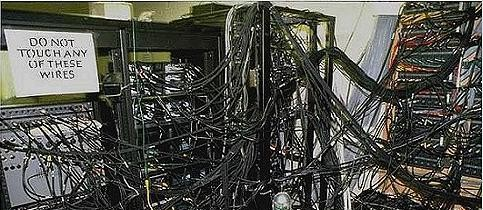
\includegraphics[height=3.5cm]{img/crazy-wiring.jpg}
\end{frame}

\subsubsection{Components for the WG Method}

\begin{frame}
  \frametitle{How Generality is Achieved: Abstraction and Modularity}
  Divide system into components having clear, limited roles.\\
  \pause
  \tcbset{colback =red!5!white, colframe =red!75!black, left=0mm,right=0mm,bottom=0mm,top=0mm}
  \begin{block}{Major Components}
    \tcbox{\shadowbox{Mesh}}
    \raisebox{1.4mm}{\shadowbox{WGrad Solver}}
    \raisebox{1.4mm}{\shadowbox{Basis}}
    \raisebox{1.25mm}{\shadowbox{Proj}}
    \tcbox{\shadowbox{VBF}}
    \raisebox{3.4mm}{\fbox{WG Solver}}
  \end{block}
  \pause
  \begin{block}{Auxiliary Types \& Components}
    \shadowbox{Monomial}
    \shadowbox{Polynomial}
    \shadowbox{Vector Monomial}
    \shadowbox{Weak Grad}
    \shadowbox{WG Solution}
    \raisebox{2mm}{\fbox{Error Norms}}
    \raisebox{2mm}{\fbox{Quadrature}}
    \raisebox{2mm}{\fbox{Linear Algebra}}
  \end{block}
  \pause
  \raisebox{-2mm}{\shadowbox{Shadowed}} components represent \emph{types}, with custom ops.\\
  \pause
  \raisebox{-2mm}{\tcbox{Enclosed}} types represent abstract
  types, or \emph{contracts}, as a set of operations which actual ``plugged in'' types must implement.
\end{frame}

\subsection{Bringing Components Together - Example}

\begin{frame}[fragile]{Bringing Components Together -- Example Run}
  \tcbset{colback =red!5!white, colframe =red!75!black, left=0mm,right=0mm,bottom=0mm,top=0mm, tcbox raise base}
  \begin{Verbatim}[gobble=4, commandchars=\\\{\}, fontsize=\small, fontfamily=tt]
    fn u(x: &[R]) -> R  \{ cos(x[0]) + sin(x[1]) \} \textcolor{gray}{// exact solution}
    fn f(x: &[R]) -> R  \{ cos(x[0]) + sin(x[1]) \} \textcolor{gray}{// var form rhs}
    fn g(x: &[R]) -> R  \{ u(x) \} \textcolor{gray}{                 // boundary cond}

    let \textcolor{green!50!black}{mesh} = \spot{~RectMesh}::new(~[0.,0.], ~[2*pi,2*pi], ~[500, 500]);

    let \textcolor{blue}{basis} = &WGBasis::new(\tcbox{\textcolor{green!50!black}{mesh}}, MaxMonDeg(3), MaxMonDeg(2));

    let \textcolor{orange!50!red}{vbf} = \spot{VBFLaplace}::new(None, \textcolor{blue}{basis});

    let wg_sol = wg_solver::solve(\tcbox{\textcolor{orange!50!red}{vbf}}, \textcolor{blue}{basis}, f, g);

    let err = err_L2_norm(u, &wg_sol);
  \end{Verbatim}
  \footnotesize {
    \textcolor{gray}{// \spot{\emph{Any} types satisfying the respective contracts are usable at these spots.}}\\
    \textcolor{gray}{// The types are only manipulated via contract-guaranteed operations within\\
      // the method -- black boxes with contract ops being the external controls.}
  }
\end{frame}


\begin{frame}[fragile]
  \frametitle{Creating Types}
  \begin{itemize}[<+->]
    \item A \emph{type} consists of some data bundled together seamlessly with the operations that act on the data.  The operations
      always come along with the data, when instances of the type are passed around between functions.  Given an \emph{instance} or
      \emph{object} named \textcolor{blue}{\small \texttt{someObject}} of a given type where the data is contained, operations on the
      type are normally denoted \textcolor{blue}{\small \texttt{someObject.\textbf{\textcolor{orange}{someFunction}}(arg1,\dots,argN)}}.

    \item We saw this above, where objects representing a mesh, a basis, and a vbf were created. It should be apparent
      that the operations must come along with these objects, because the WG method only receives these objects to its solve function, and yet
      somehow also must be getting the operations for the specific mesh and VBF.
      \tcbset{colback =red!5!white, colframe =red!75!black, left=0mm,right=0mm,bottom=0mm,top=0mm, tcbox raise base}
      \begin{Verbatim}[gobble=6, commandchars=\\\{\}, fontsize=\scriptsize, fontfamily=tt]
        let \textcolor{green!50!black}{mesh} = ~RectMesh::new(~[0.,0.], ~[2*pi,2*pi], ~[500, 500]);
        let \textcolor{blue}{basis} = &WGBasis::new(\tcbox{\textcolor{green!50!black}{mesh}}, MaxMonDeg(3), MaxMonDeg(2));
        let \textcolor{orange!50!red}{vbf} = VBFLaplace::new(None, \textcolor{blue}{basis});
        let wg_sol = wg_solver::solve(\tcbox{\textcolor{orange!50!red}{vbf}}, \textcolor{blue}{basis}, f, g);
      \end{Verbatim}
  \end{itemize}
\end{frame}


\section{Concepts}

\subsection{Mesh Elements}

\subsubsection{Oriented Shapes}

% TODO: Not enough room on this slide! Split into two slides.  Then can go into a little more detail about how the division into sides
% is included in the idea of oriented shape.
\begin{frame}
  \frametitle{Oriented Shapes}
  \begin{columns}
    \column{.50\textwidth}
      \frame{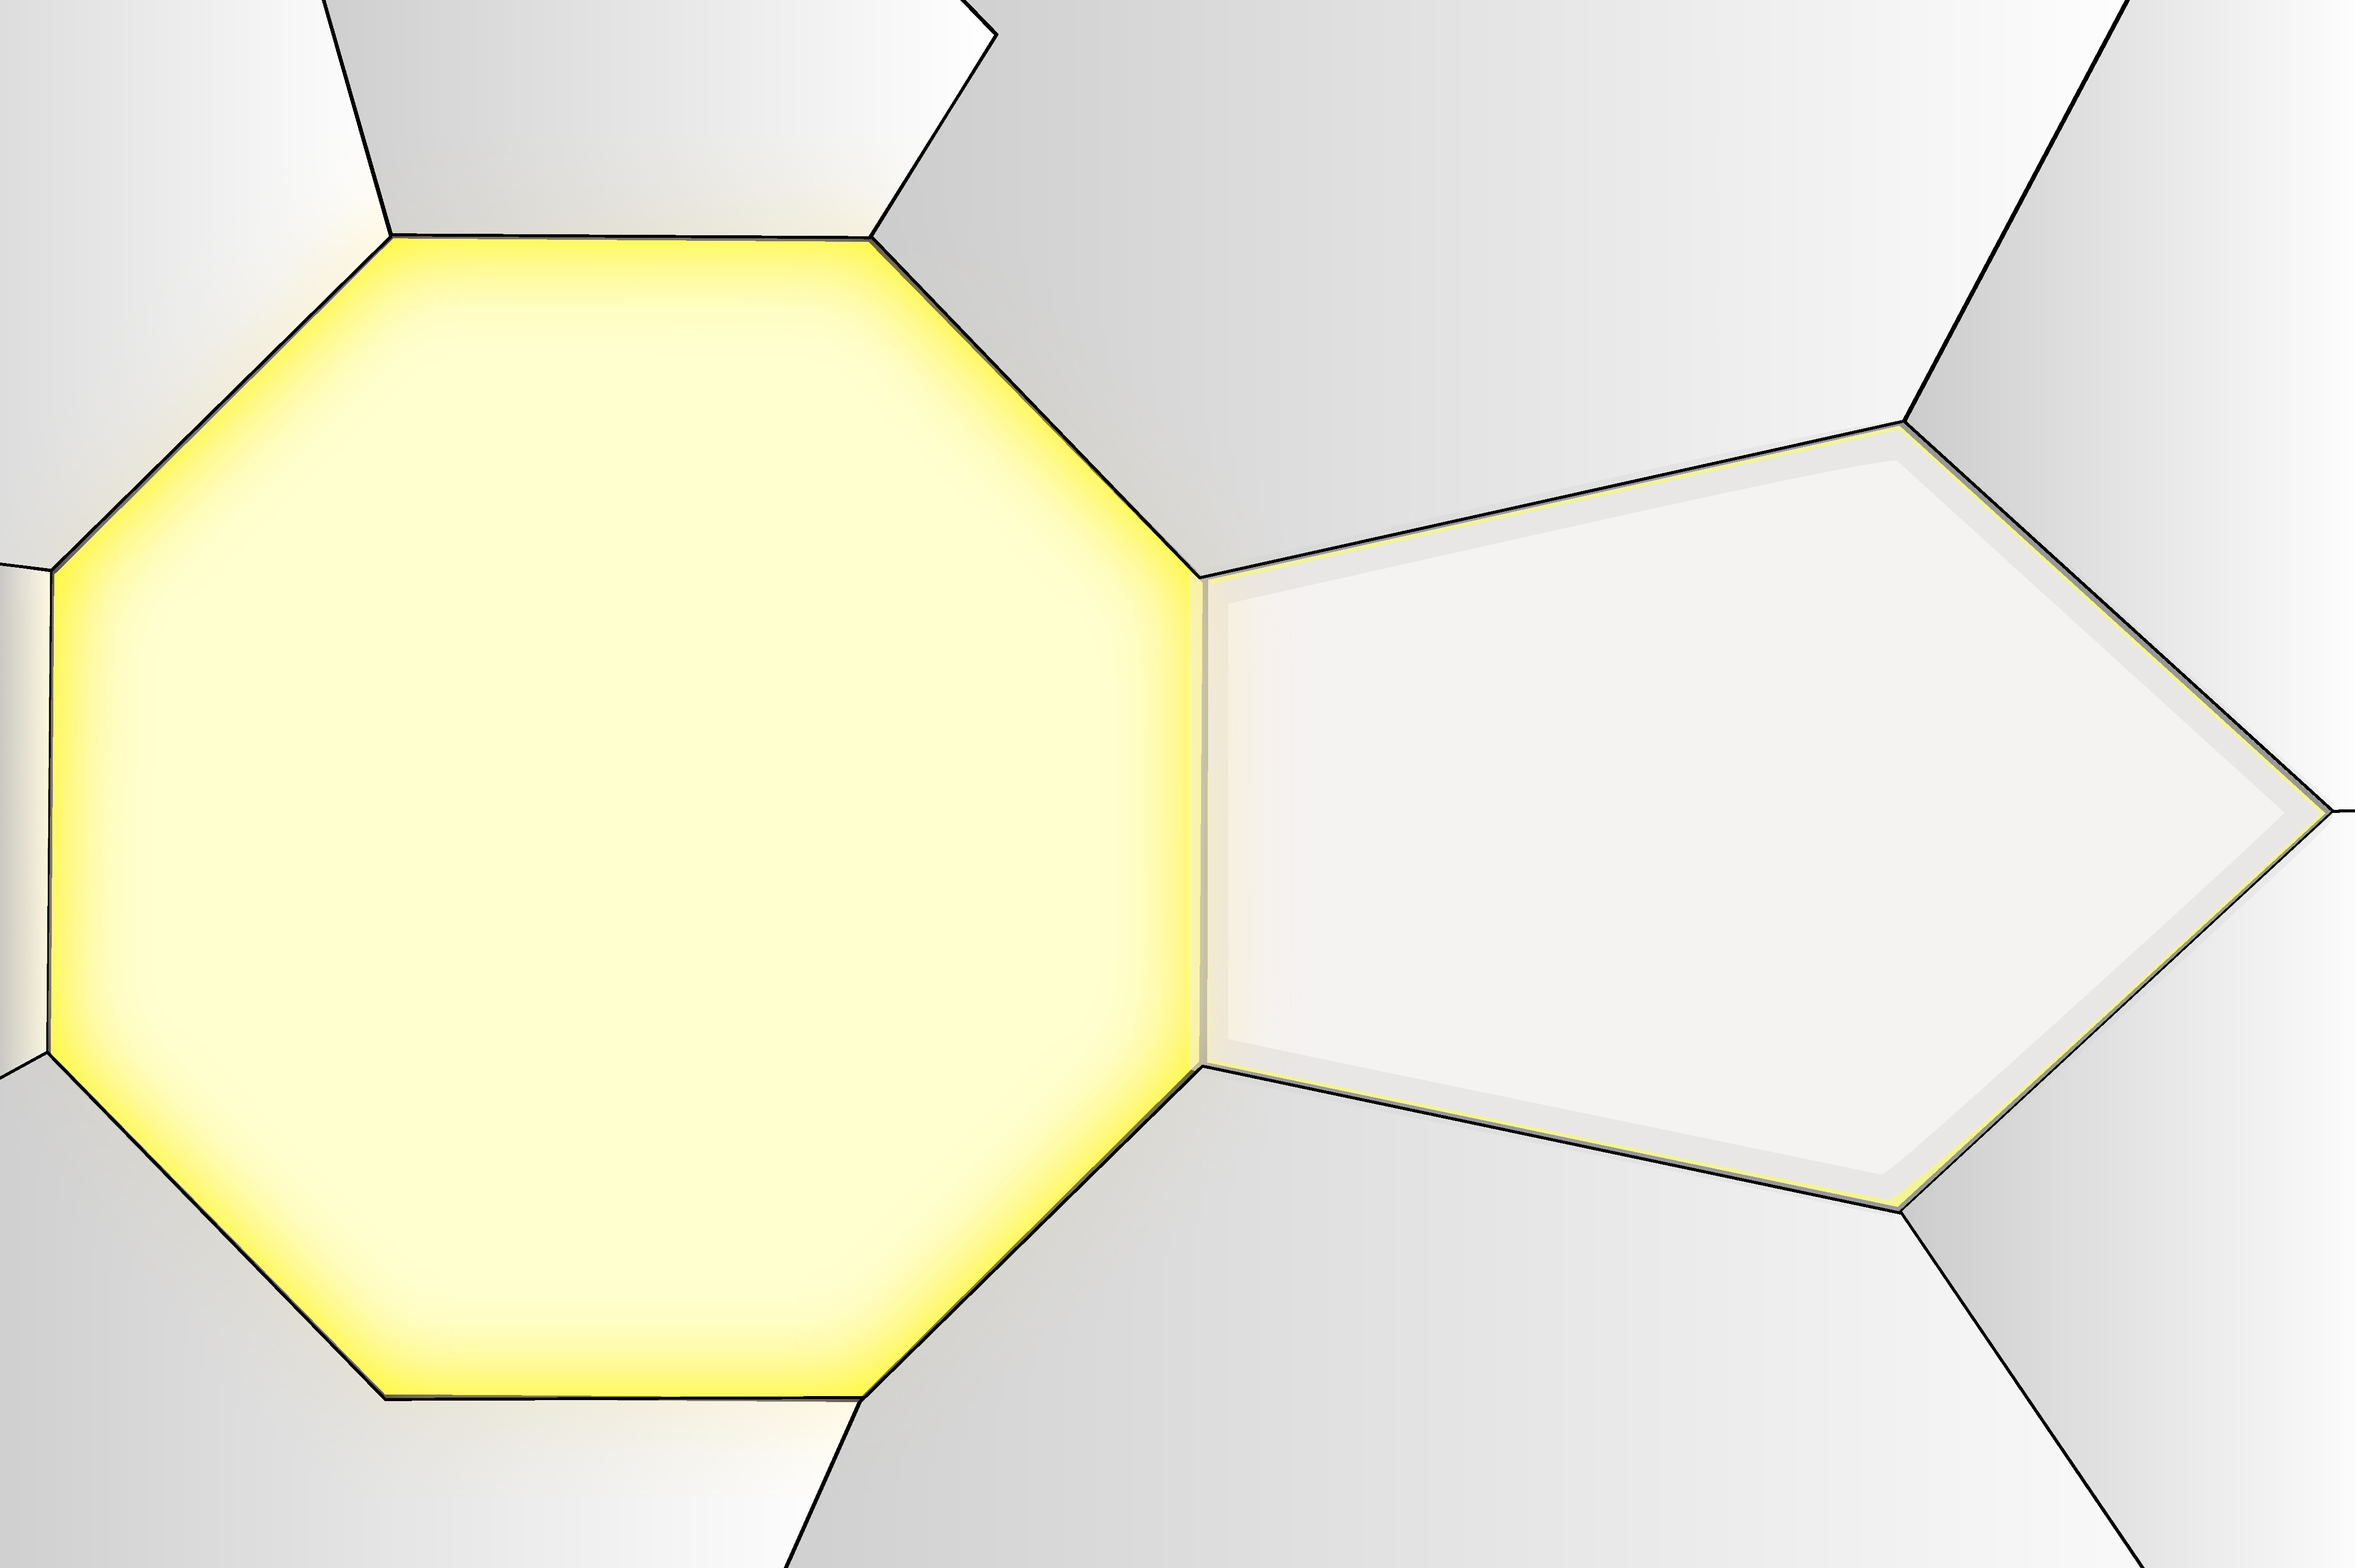
\includegraphics[width=6cm, height=4cm]{img/two_fes.pdf}}
    \column{.50\textwidth}
      \pause
      \begin{itemize}[<+->]
        \item Elements may have, \emph{independently} of each other, any \textbf{shape}, \textbf{orientation}, and \textbf{number of sides}.
        \item Two elements are of the same \textbf{\emph{oriented shape}} iff some translation takes each side of one onto
          a matching side of the other.
      \end{itemize}
  \end{columns}
  
  \begin{itemize}[<+->]
    \item Is an abstraction of a finite element, ignoring its position, but including its division into sides (for ``hanging nodes'').
%    \item Many calculations can be done on an oriented shape instead of individual on elements.
    \item Mesh must assign an oriented shape for \emph{each} finite element. 
    \item Mesh will identify oriented shapes by enumerating them in some order of its choosing. Are just \emph{opaque} identifiers to other comps.
%      Enumeration makes iteration and use as an array index easy. Mesh internally can store more information.
  \end{itemize}
\end{frame}

\subsubsection{Identifying Finite Elements and Non-Boundary Sides}

\begin{frame}
  \frametitle{Identifying Finite Elements and Non-Boundary Sides}
  \begin{columns}
    \column{.50\textwidth}
      \begin{itemize}[<+->]
        \item Mesh will need to provide identifiers for the \emph{\textbf{support faces}} for the basis shape functions.
        \item Interiors and non-boundary sides will host shape functions, so need to be identified.
      \end{itemize}
    \column{.50\textwidth}
      \alt<-2> {\frame{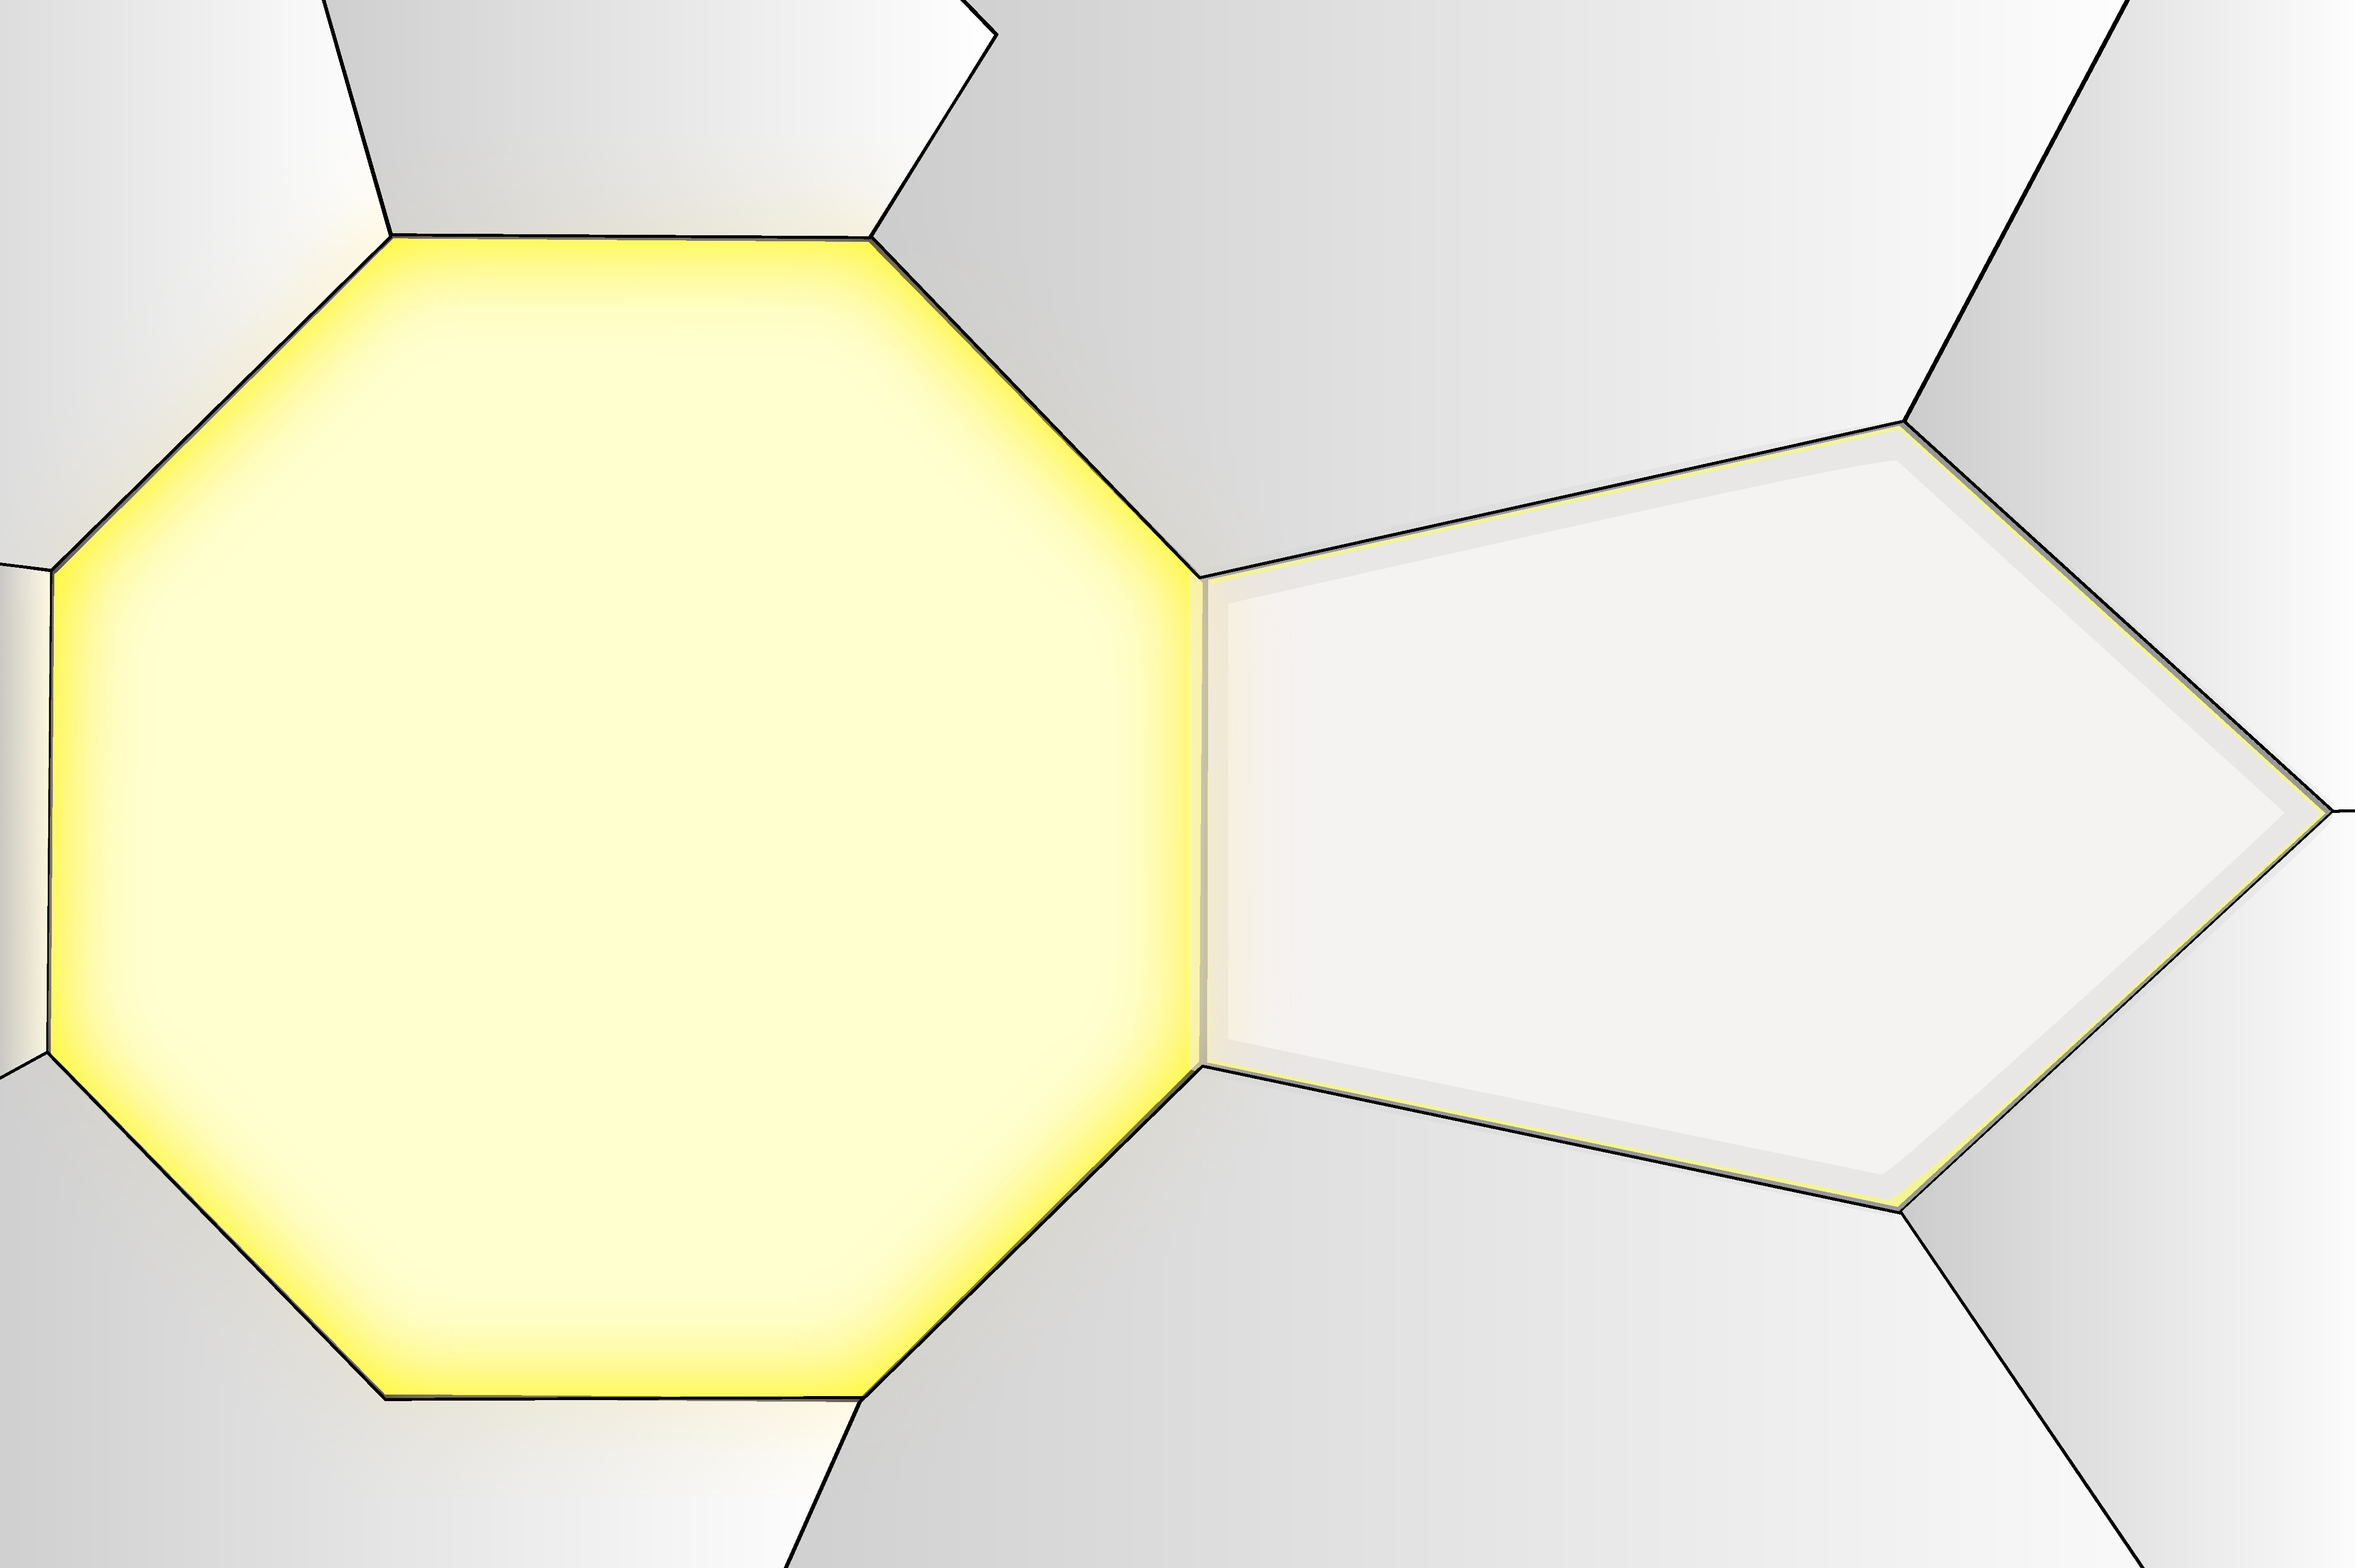
\includegraphics[width=6cm, height=4cm]{img/two_fes.pdf}}}
               {\frame{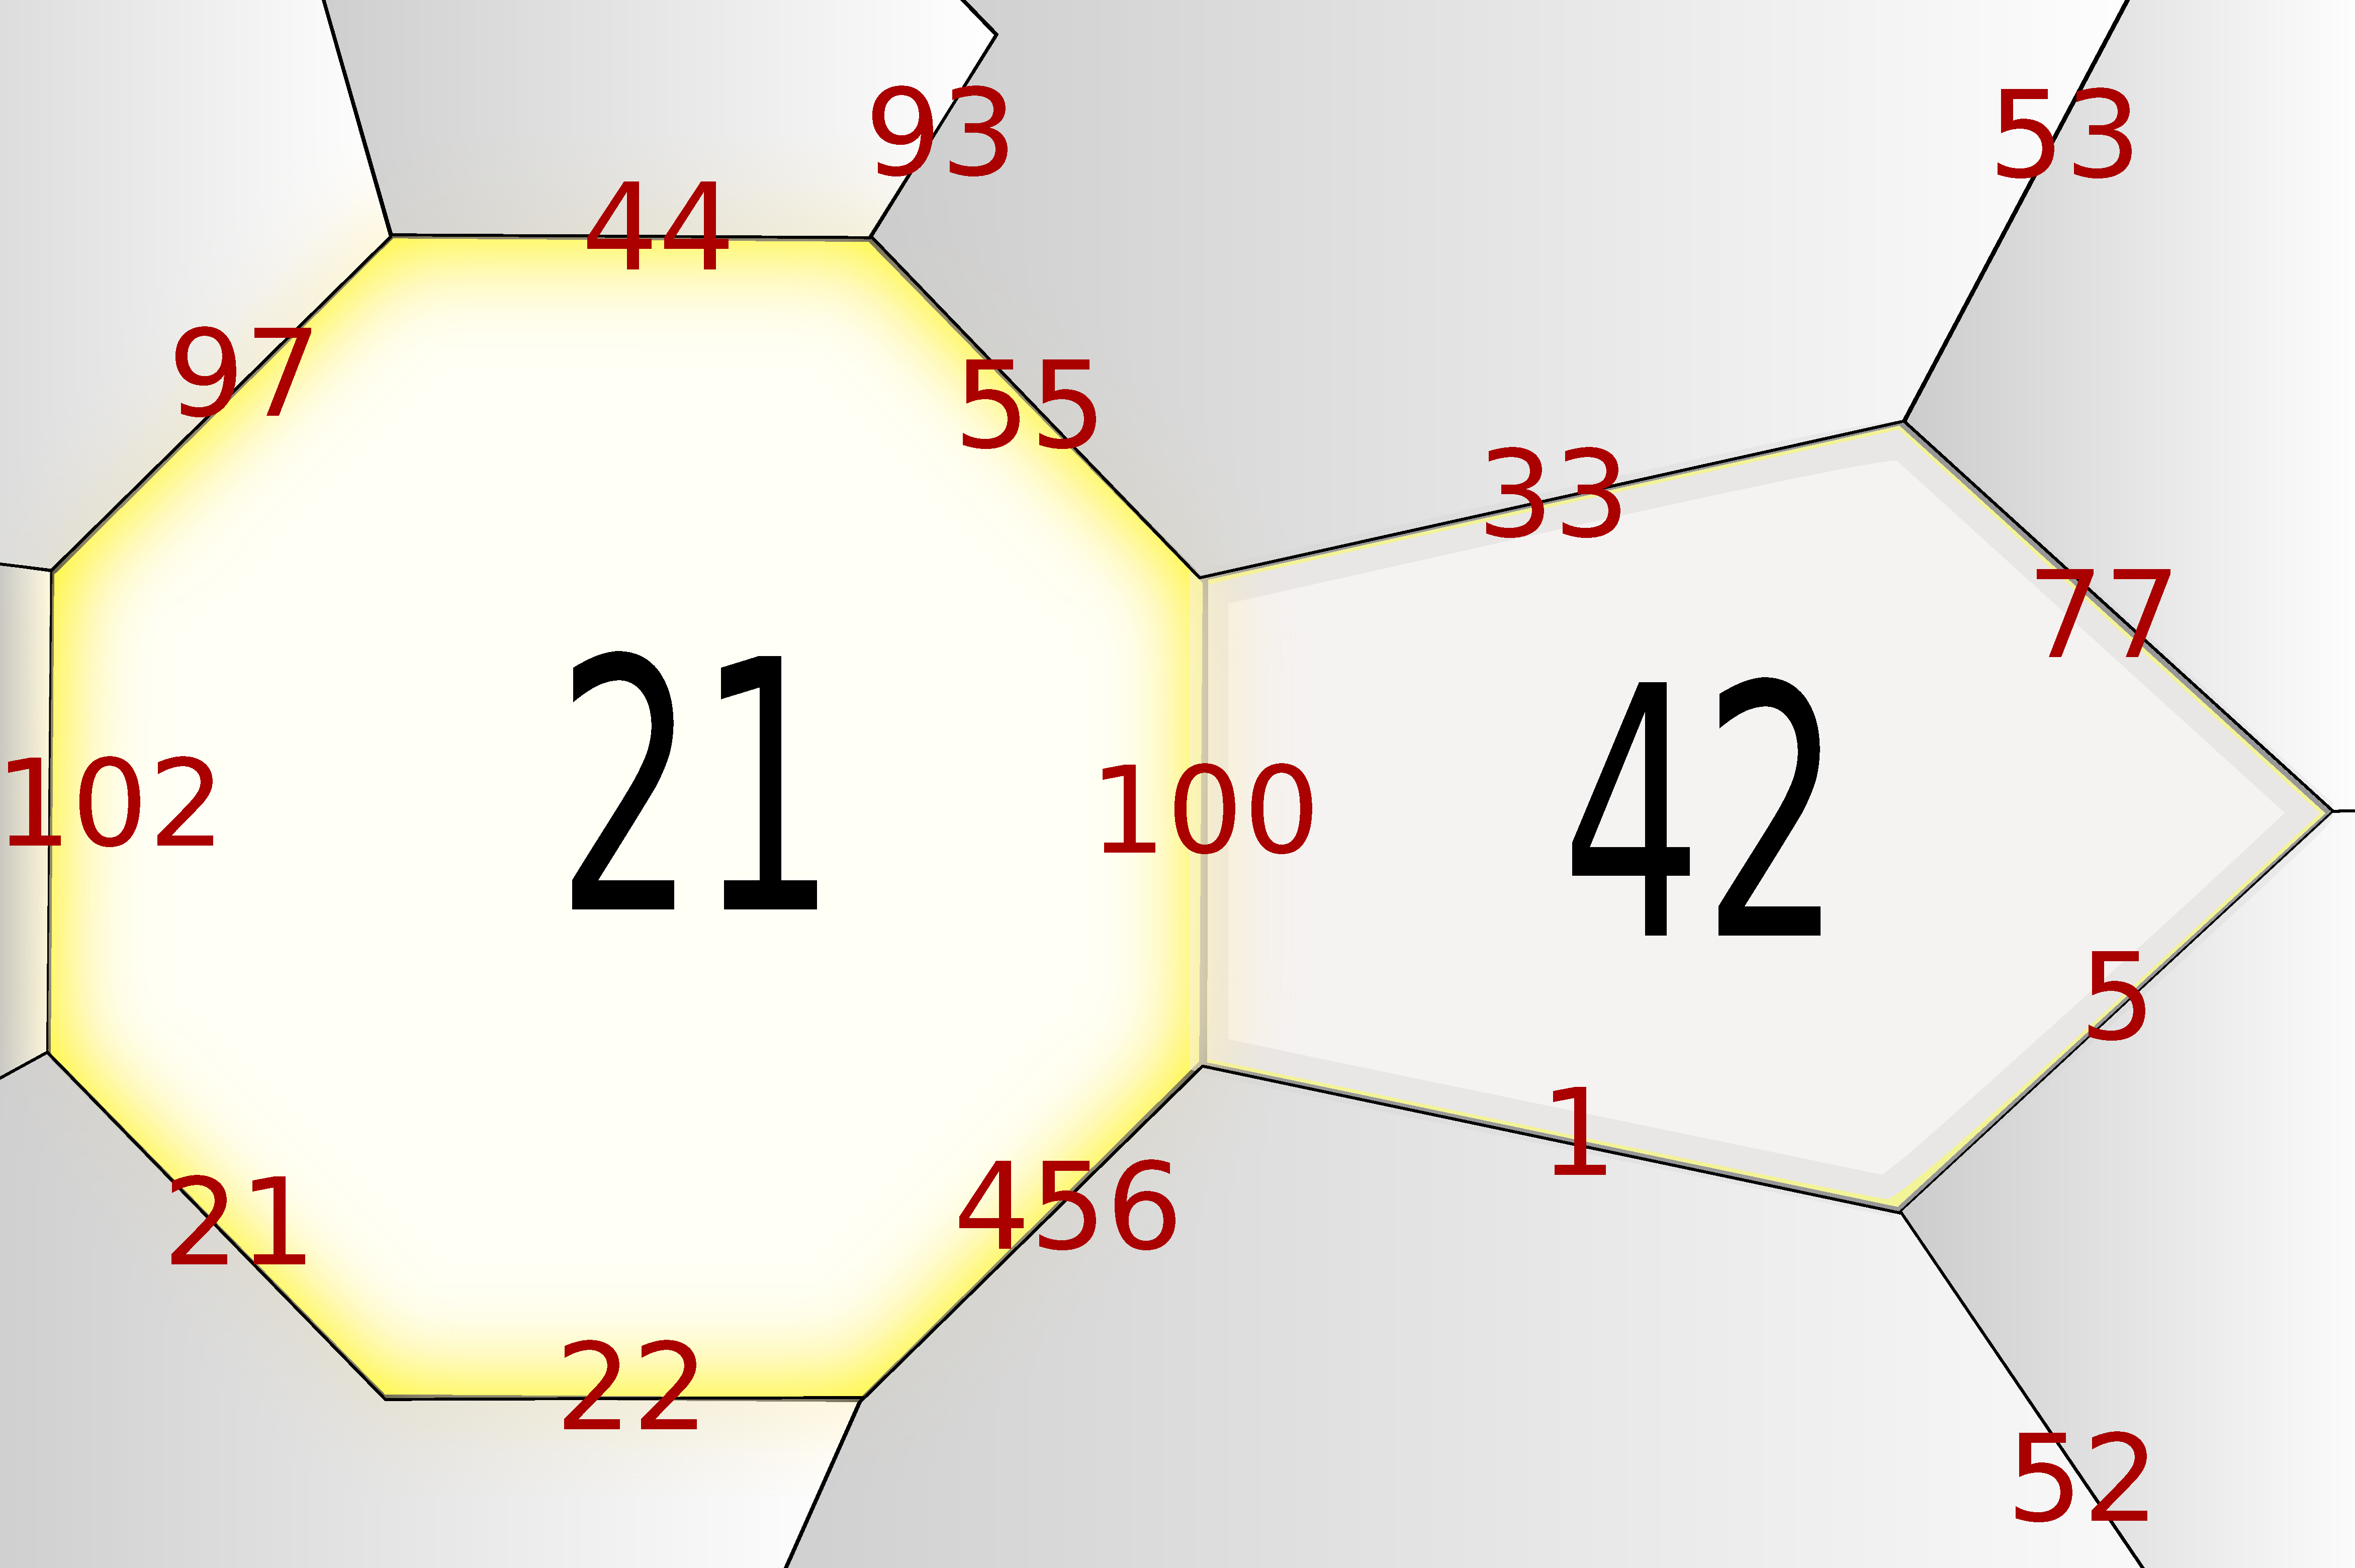
\includegraphics[width=6cm, height=4cm]{img/two_fes_enum_supp_faces.pdf}}}
  \end{columns}
  \begin{itemize}[<+->]
    \item Mesh will \textbf{enumerate finite elements (equiv., \emph{interiors}) and non-boundary sides separately}, in any order it chooses for each.
    \item Separate enumerations allow sides or fes/interiors to be dealt with separately by other components.
    \item To other components, the interior and nb side numbers are just opaque identifiers -- must ask the mesh for interpretation.
  \end{itemize}
\end{frame}
 
\subsubsection{Side Faces -- Shape Relative Side Identifiers}

\begin{frame}
  \frametitle{Side Faces -- Shape Relative Side Identifiers}
  \begin{columns}
    \column{.50\textwidth}
      \begin{itemize}[<+->]
        \item Side identifiers discussed so far are \emph{global}, and do not tell the \emph{\textbf{role}} that the side plays
          in the context of a \emph{\textbf{single oriented shape or element}}.
        \item The shape-relative side identifier is the \emph{\textbf{side face}}.
      \end{itemize}
    \column{.50\textwidth}
      \alt<-1> {\frame{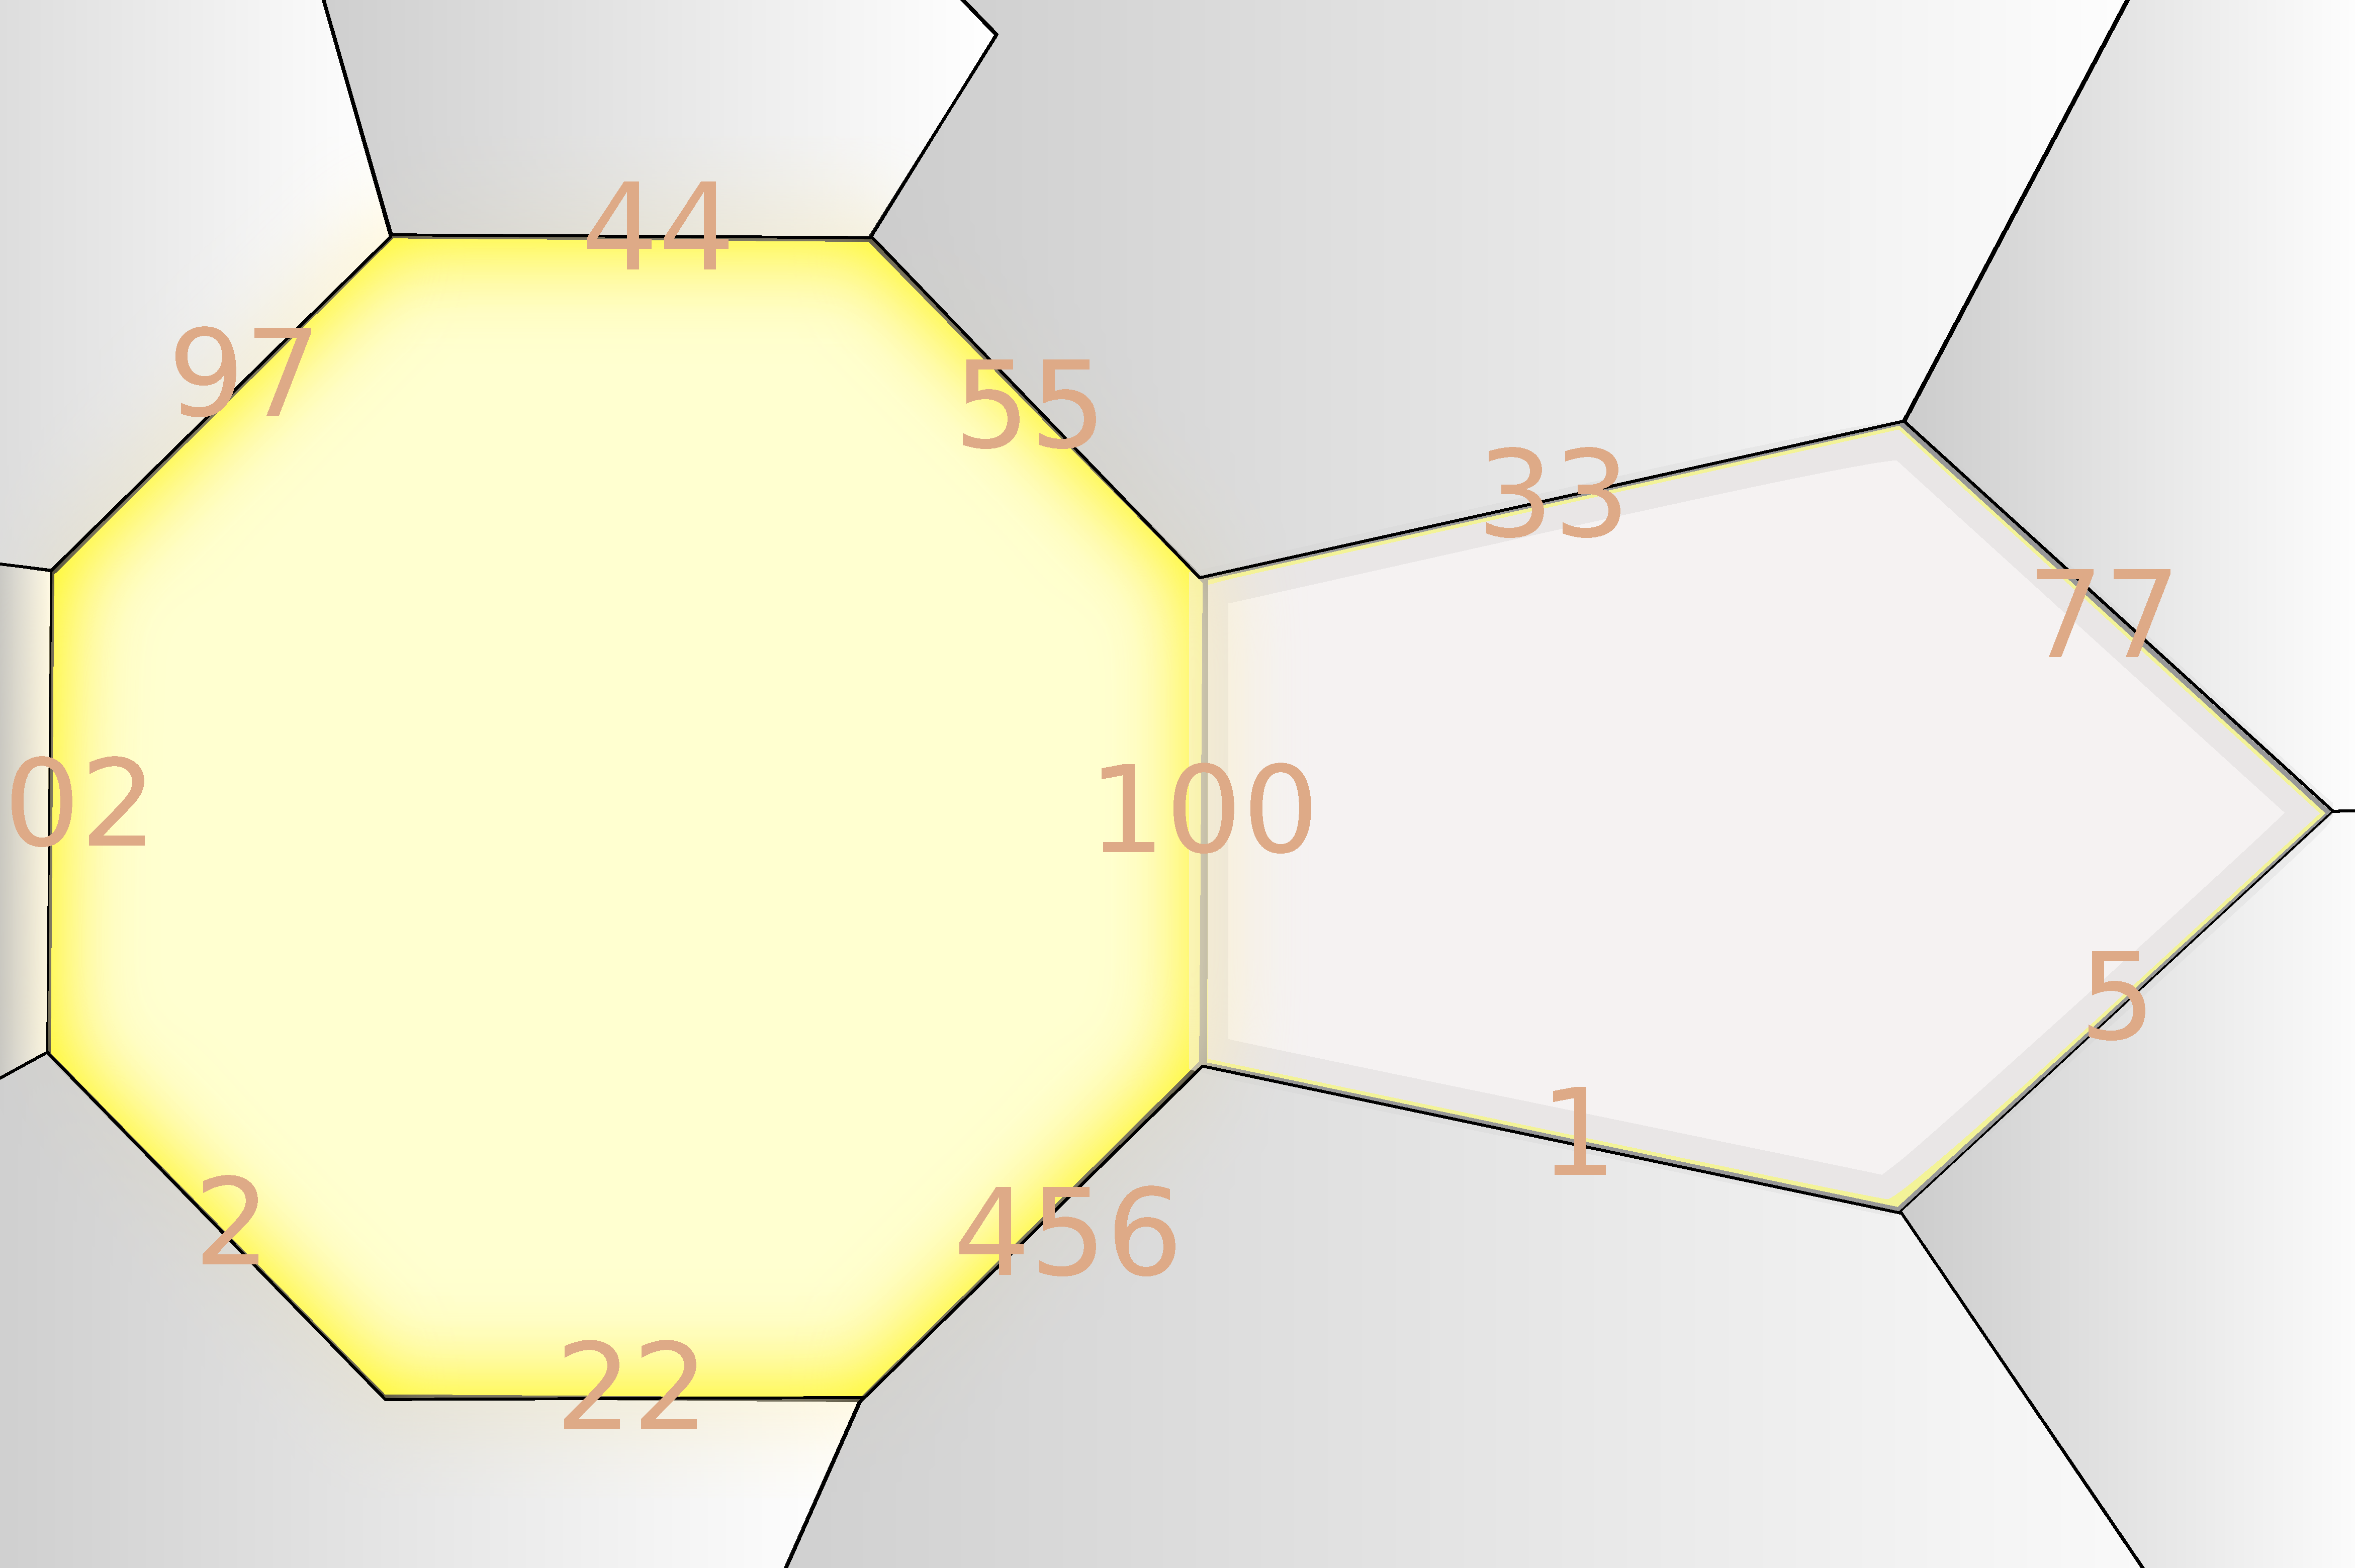
\includegraphics[width=6cm, height=4cm]{img/two_fes_enum_nb_side_nums_greyed.pdf}}}
               {\frame{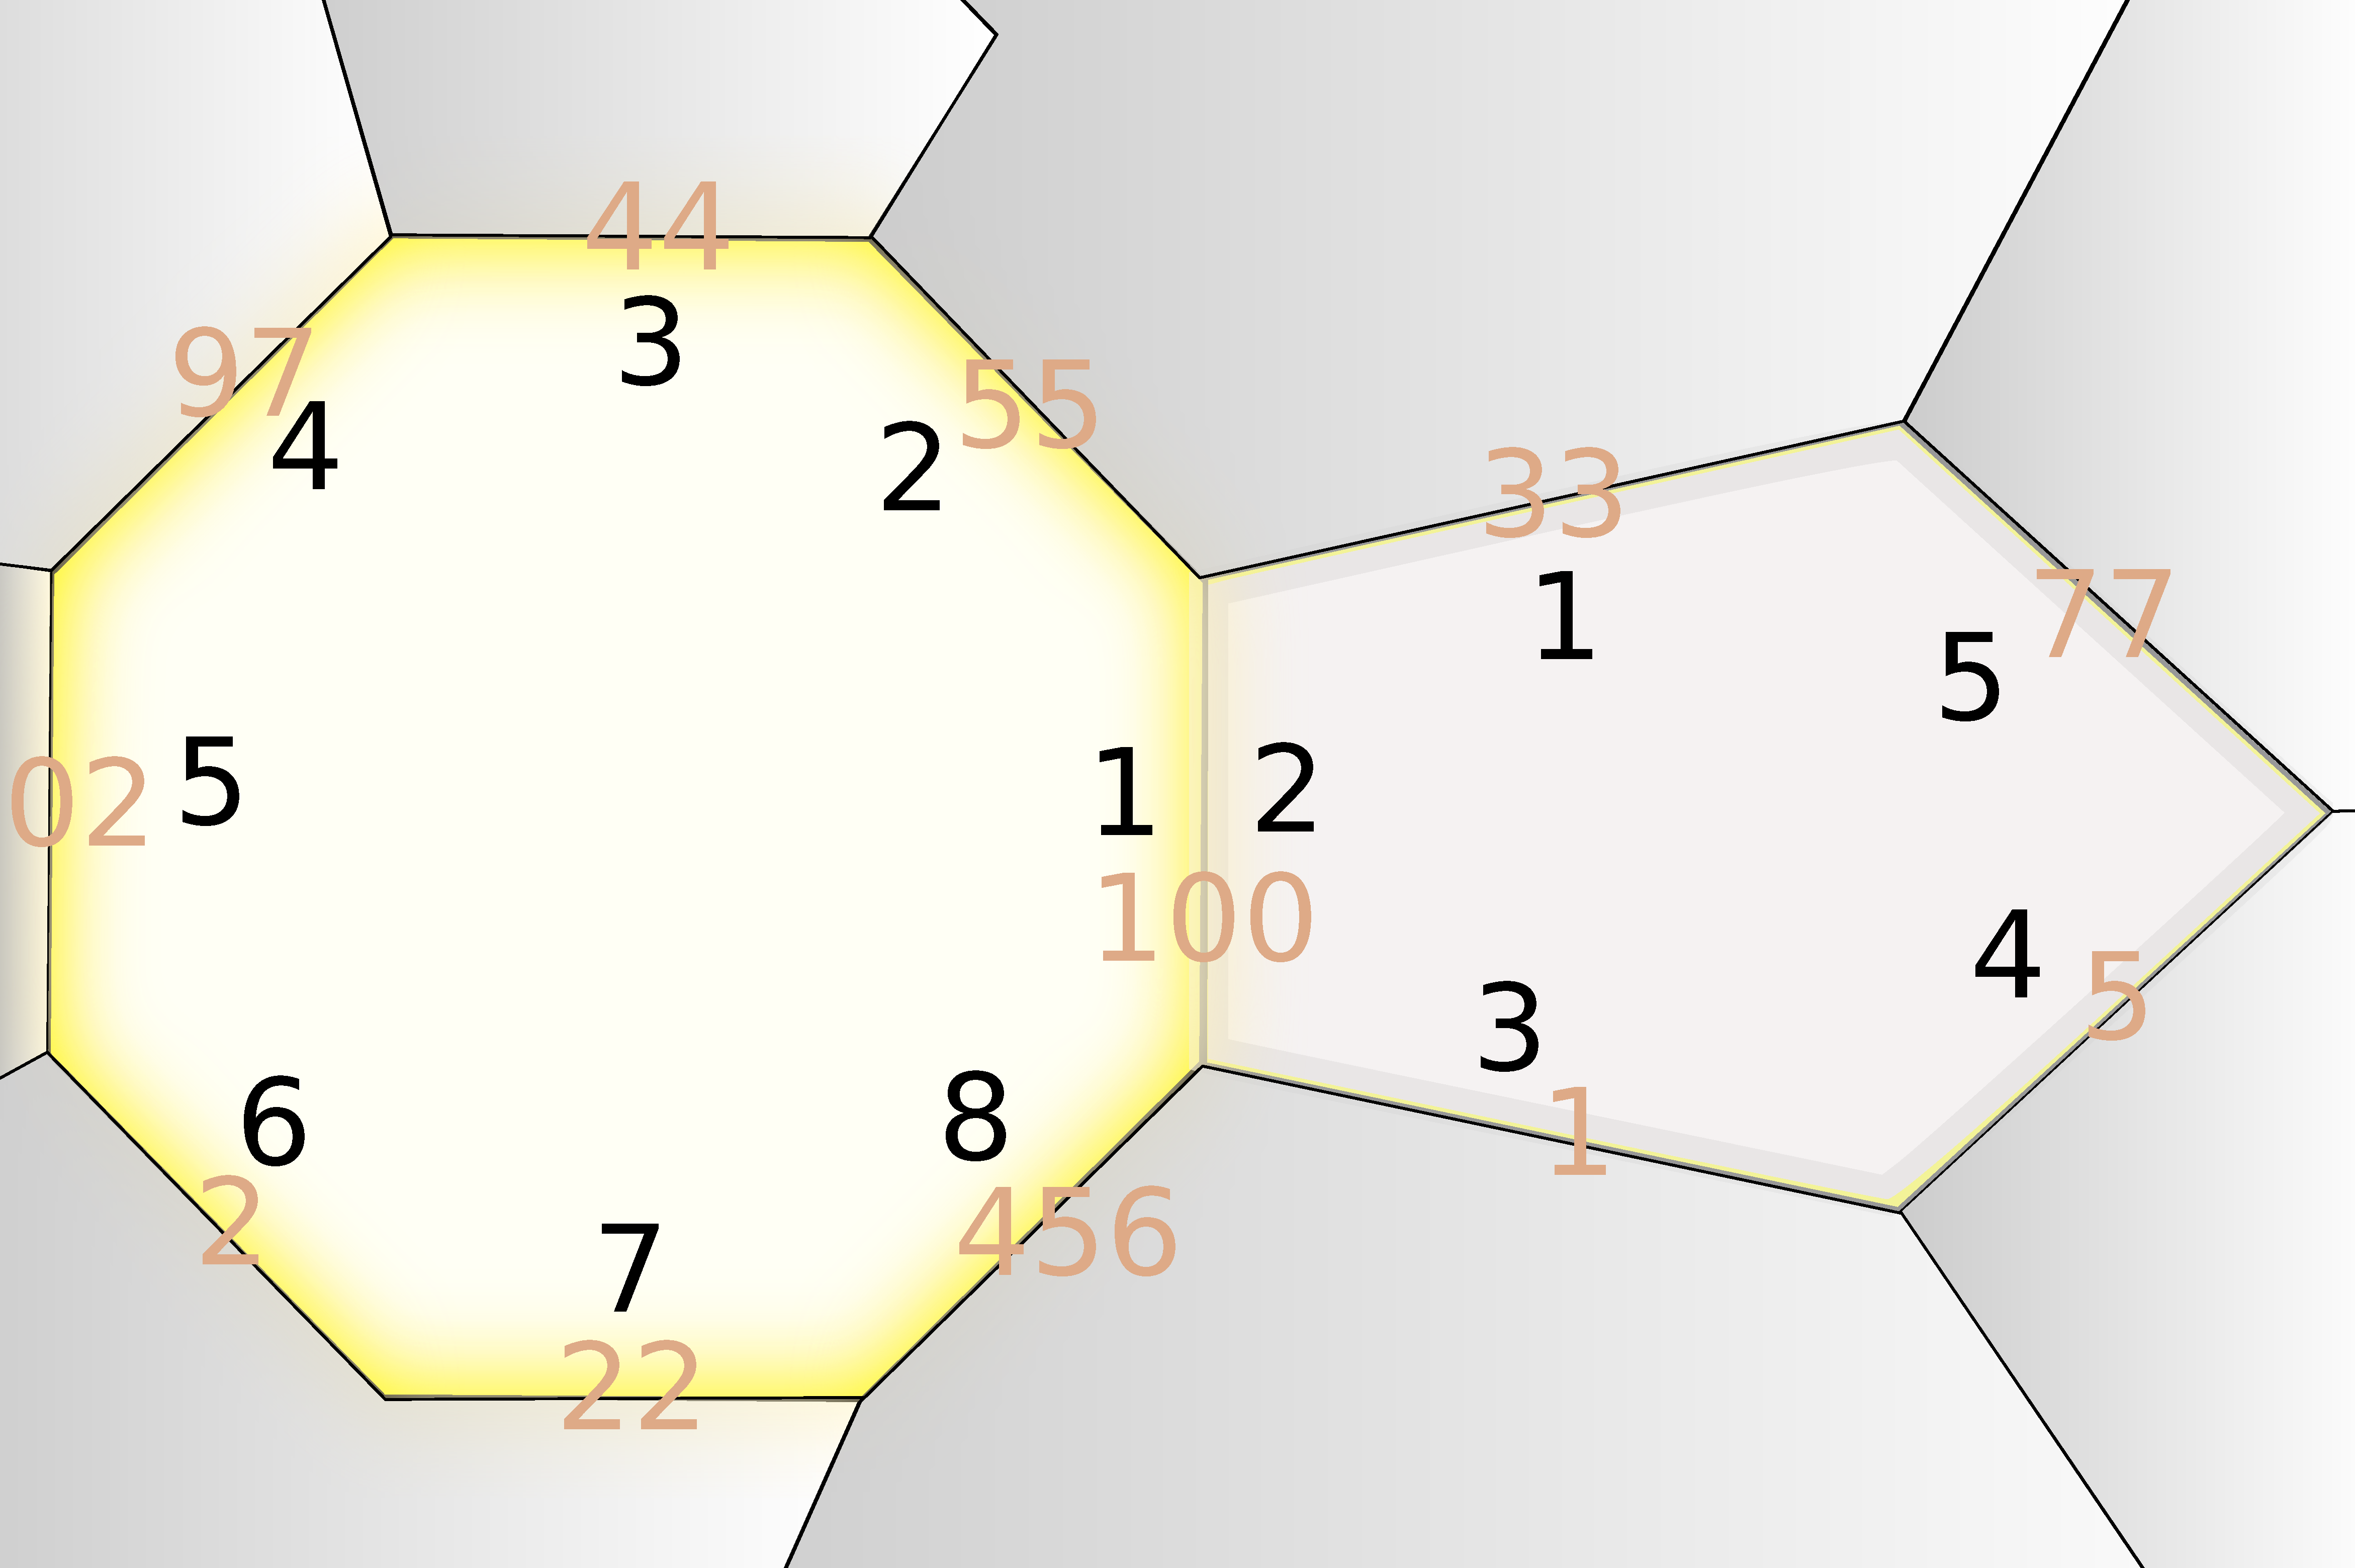
\includegraphics[width=6cm, height=4cm]{img/two_fes_enum_side_faces_nb_side_nums_greyed.pdf}}}
  \end{columns}
  \begin{itemize}[<+->]
    \item The sides may be numbered in any order by the mesh, each oriented shape having its own numbering of its side faces.
    \item A finite element inherits side face numbers from the corresponding sides of its oriented shape.
    \item Side faces are necessary to represent sides in computations involving geometry on oriented shapes and finite elements.
  \end{itemize}
\end{frame}
 
\subsubsection{Elements Including a Non-Boundary Side}

\begin{frame}
  \frametitle{Finite Elements Including a Non-Boundary Side}
  \begin{columns}
    \column{.50\textwidth}
      \begin{itemize}[<+->]
        \item Meshes will be such that each nb side is included in exactly two finite elements,
          and has no measure in any other elements.
        \item When a \emph{hanging node} divides a straight section, sections between vertexes must be separate sides.
      \end{itemize}
    \column{.50\textwidth}
    \alt<-1> {
        \frame{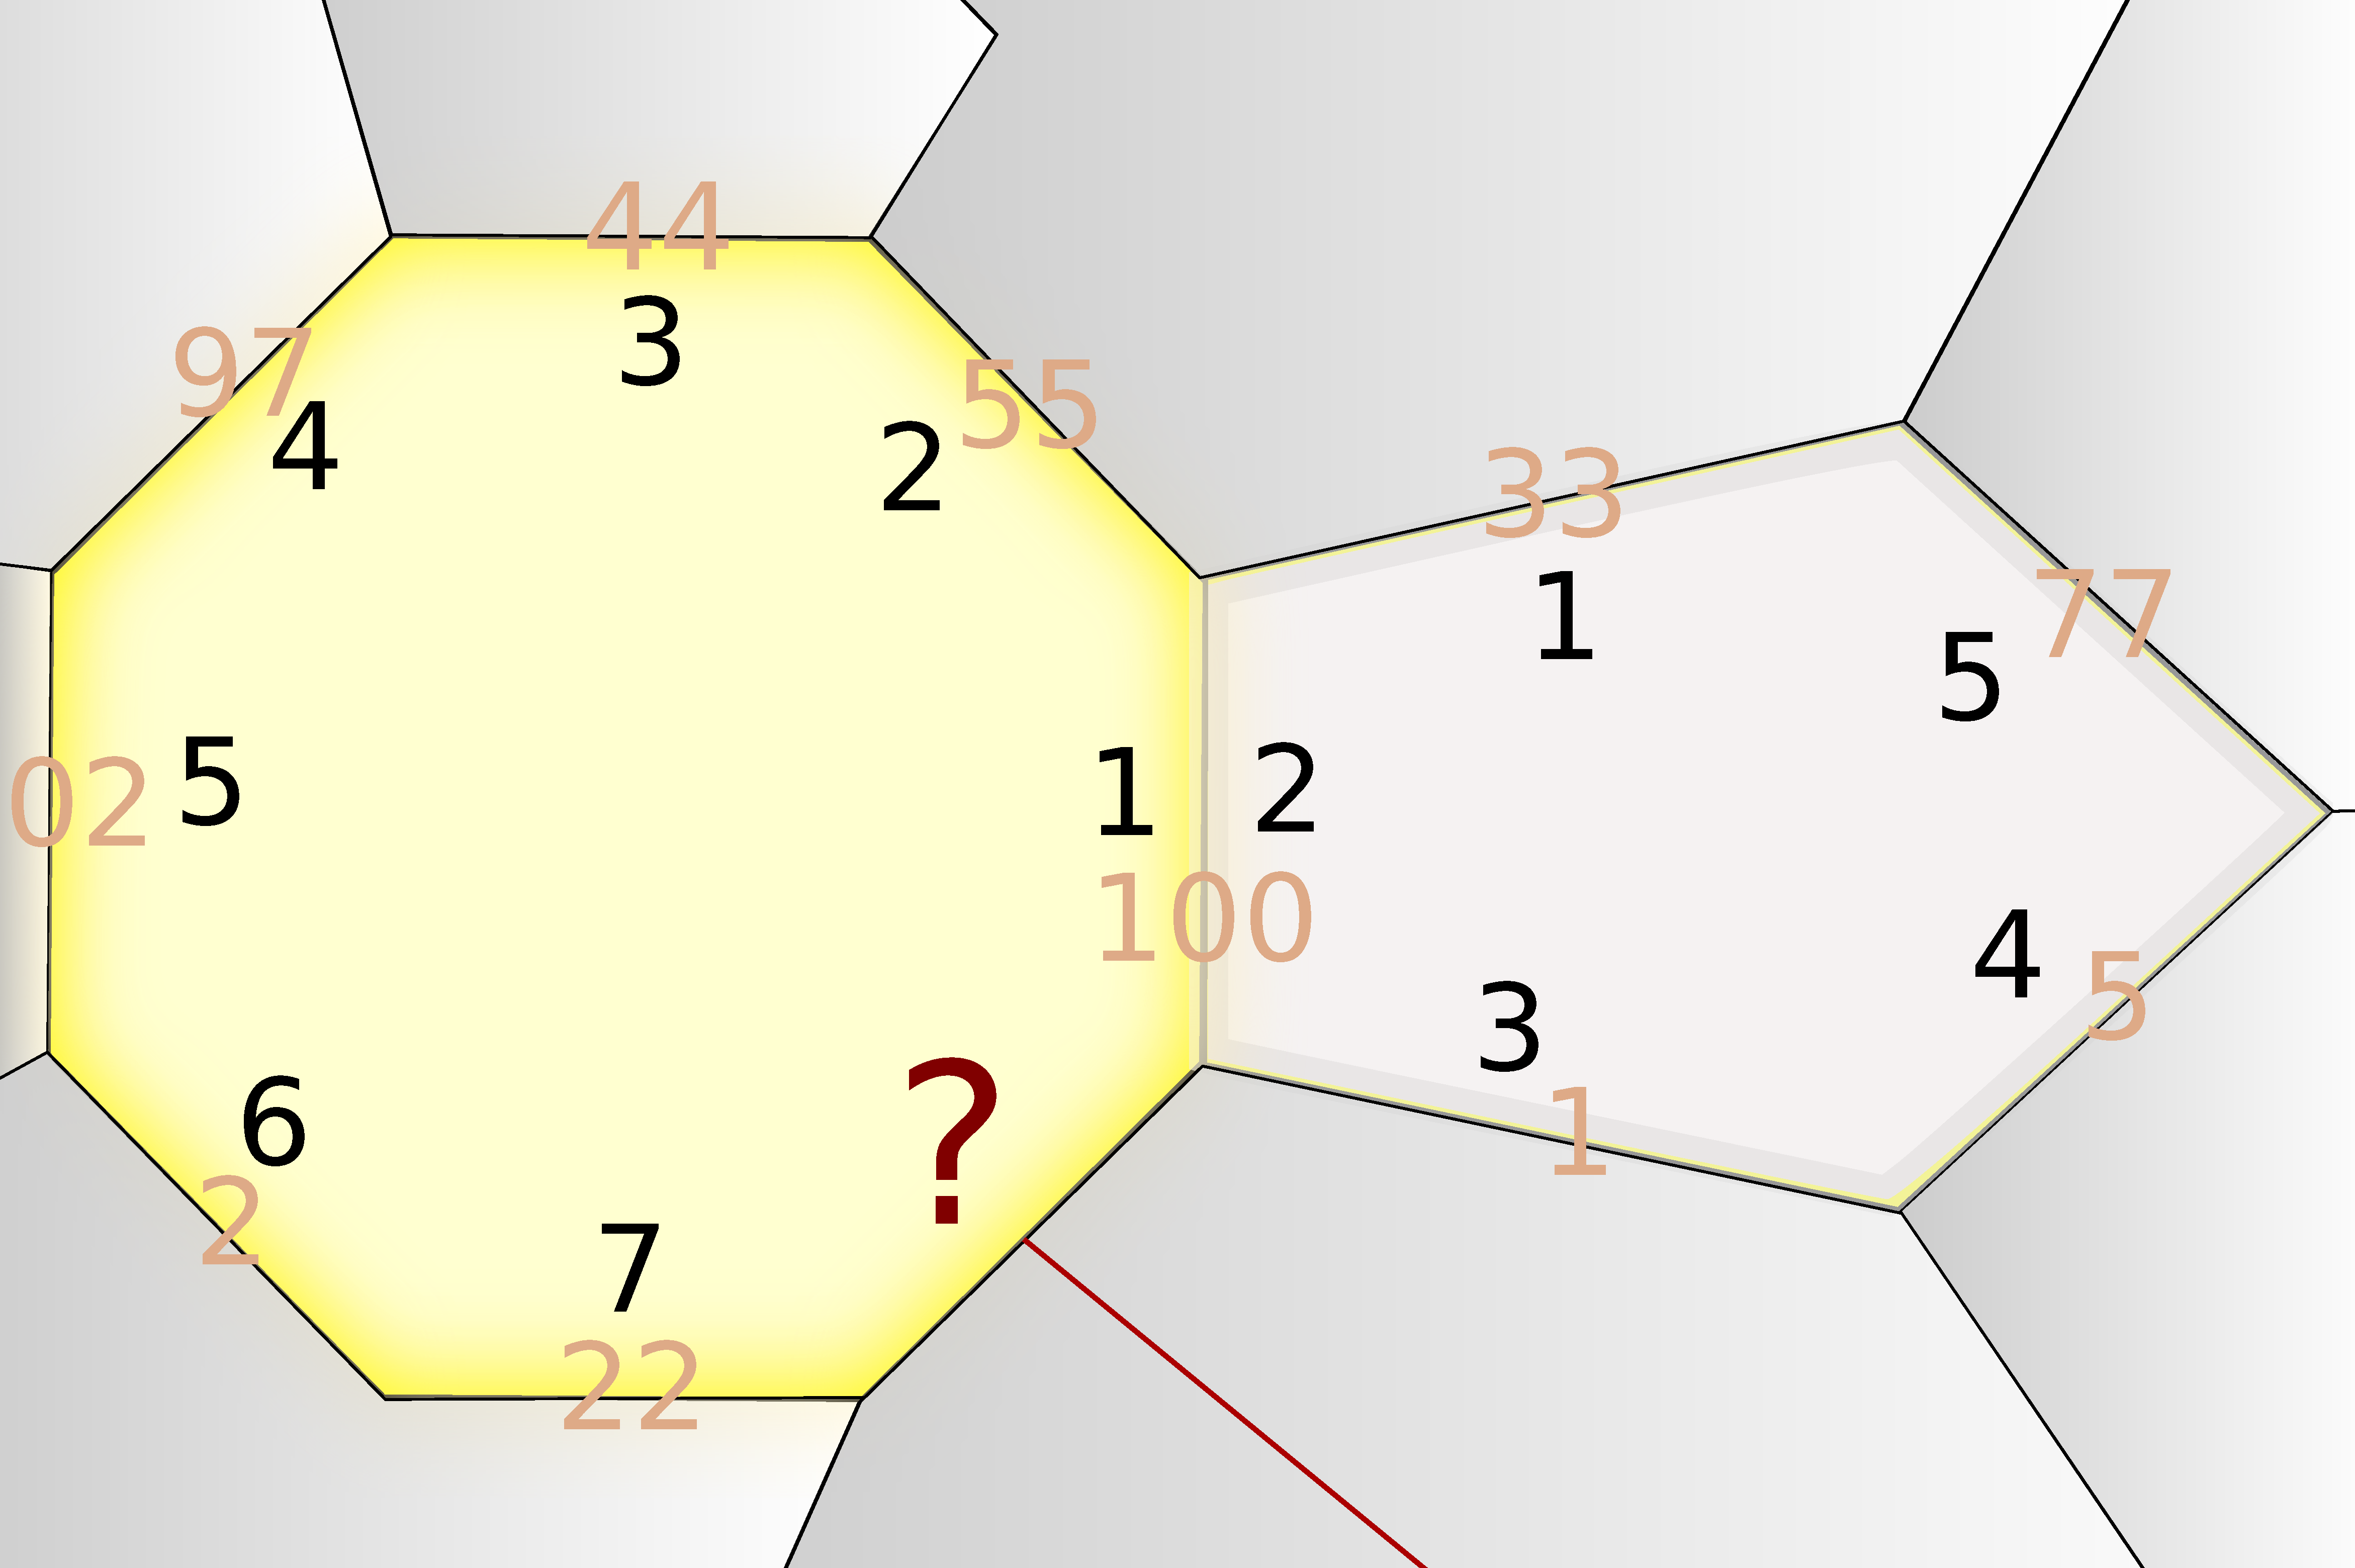
\includegraphics[width=6cm, height=4cm]{img/two_fes_hanging_node_qmark.pdf}}
      } {
        \alt<-2> {\frame{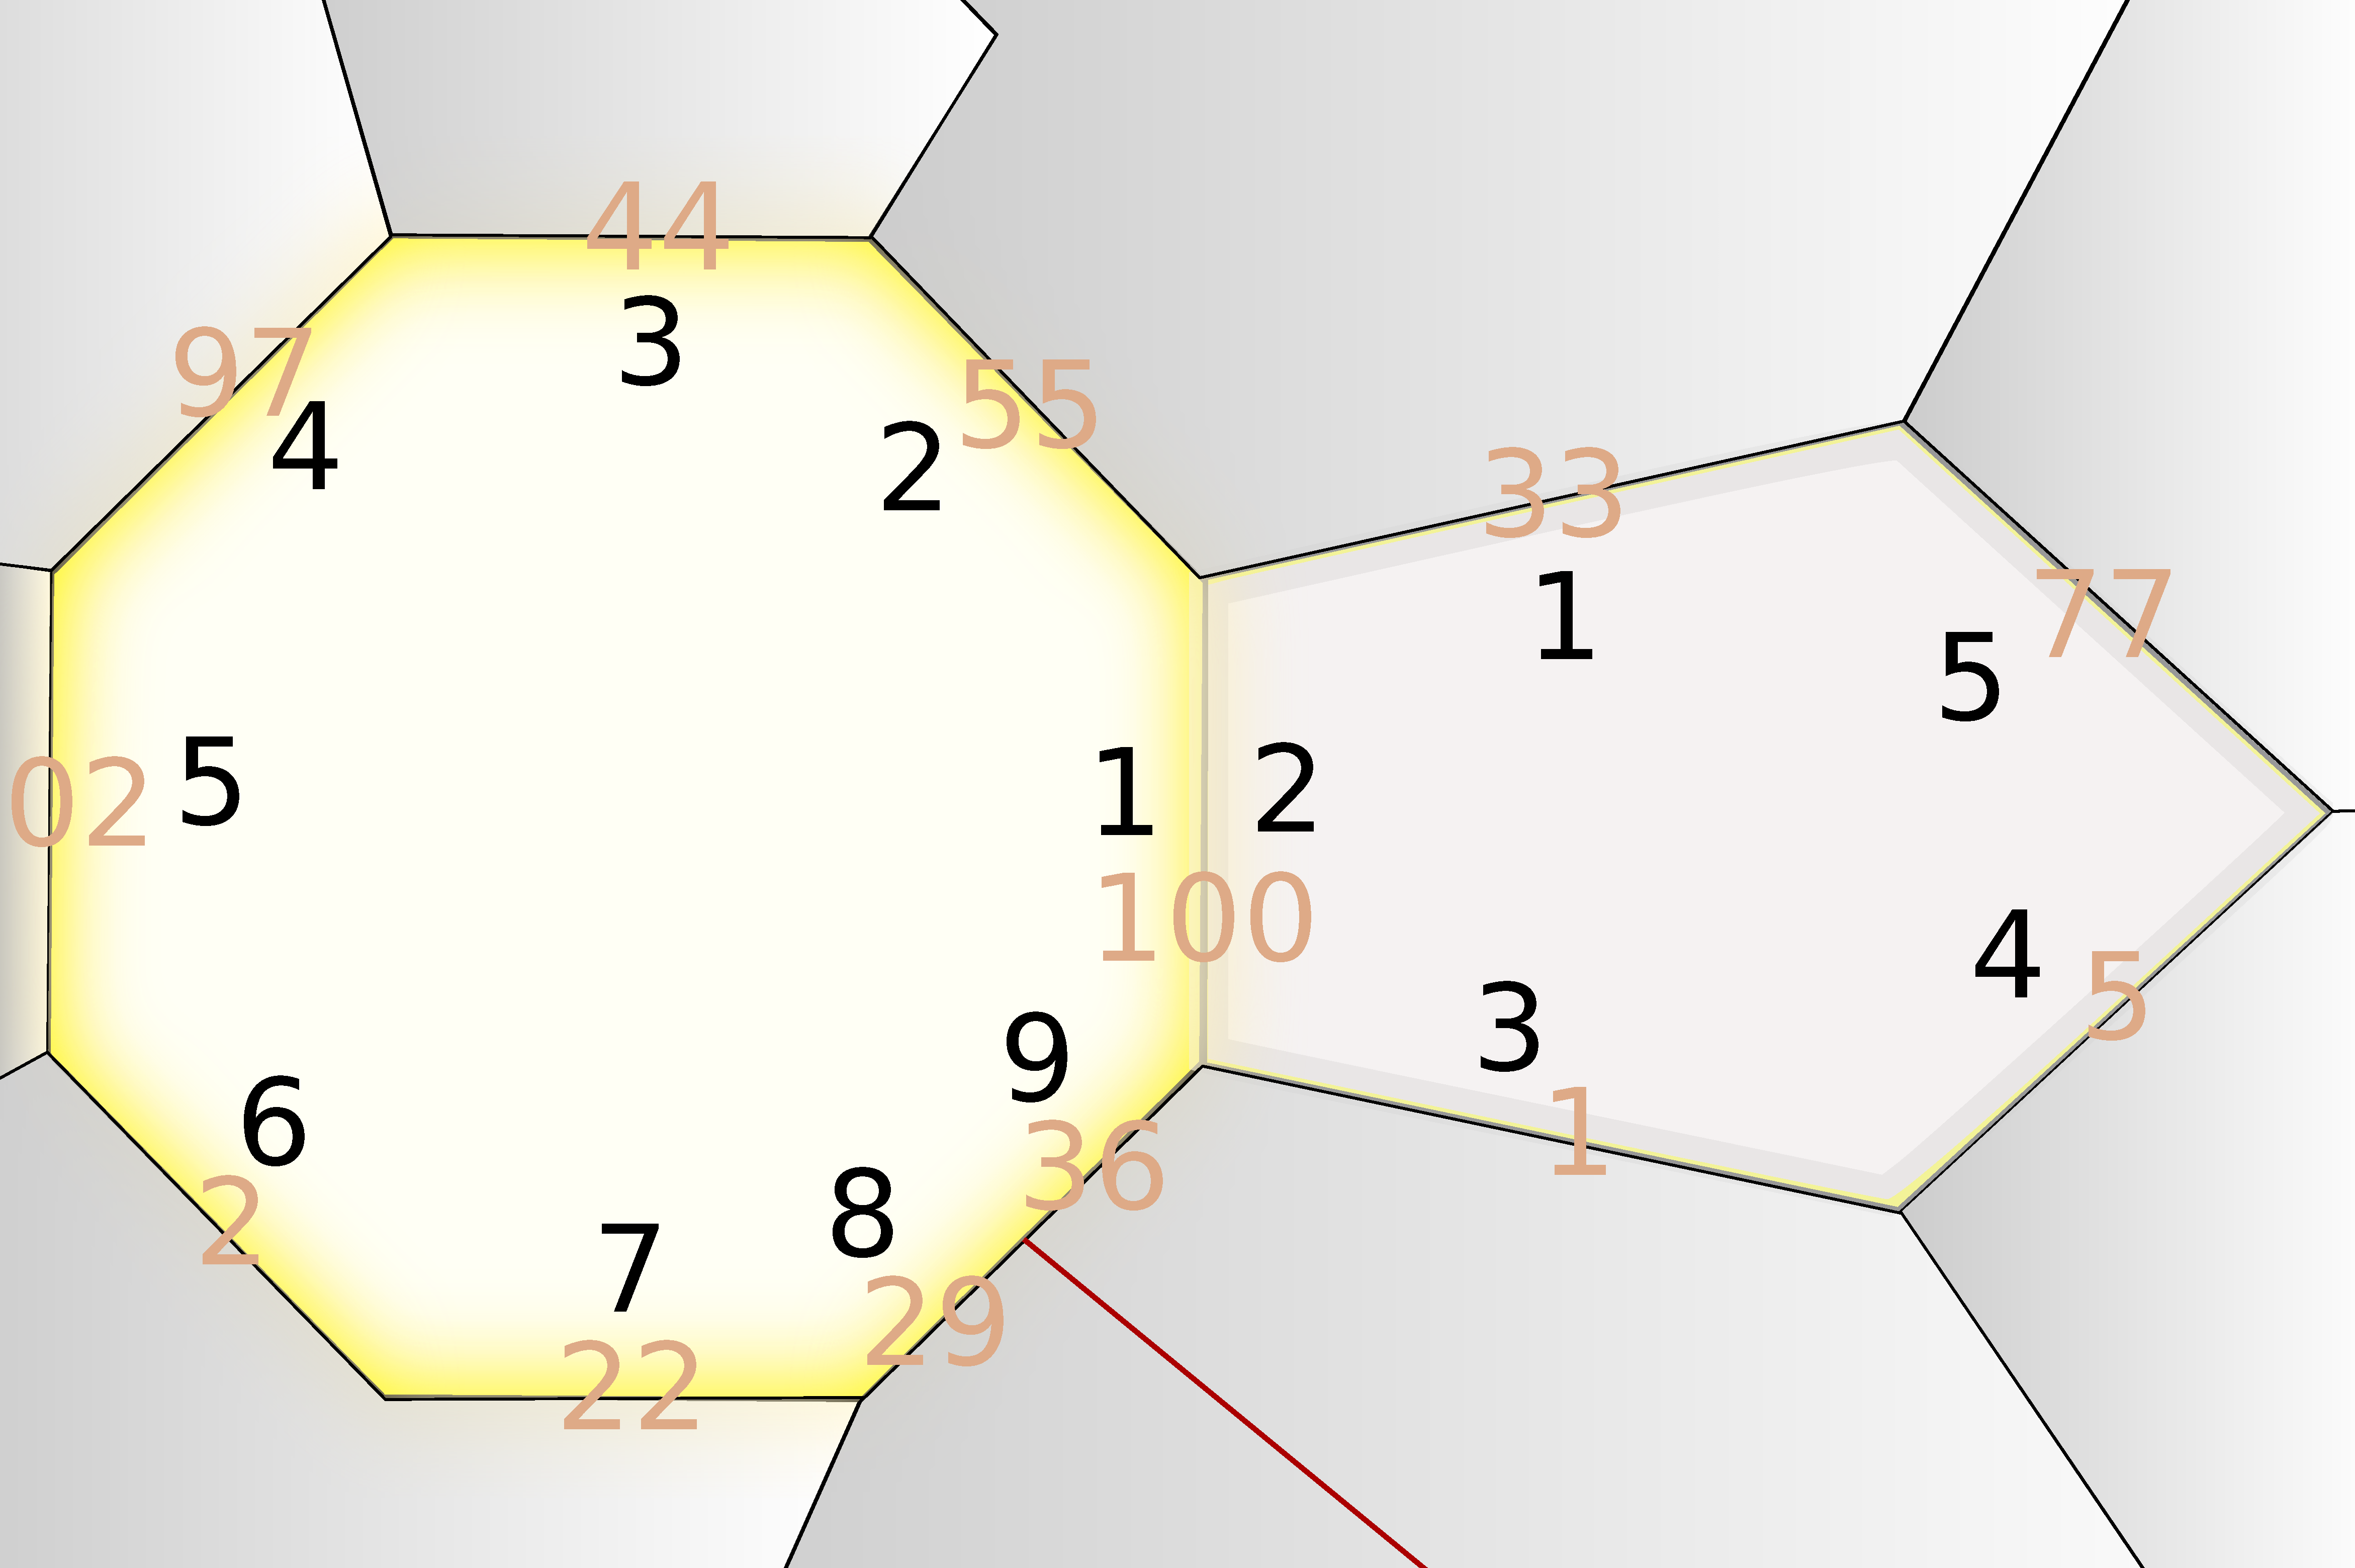
\includegraphics[width=6cm, height=4cm]{img/two_fes_hanging_node_resolved.pdf}}}
                 {\frame{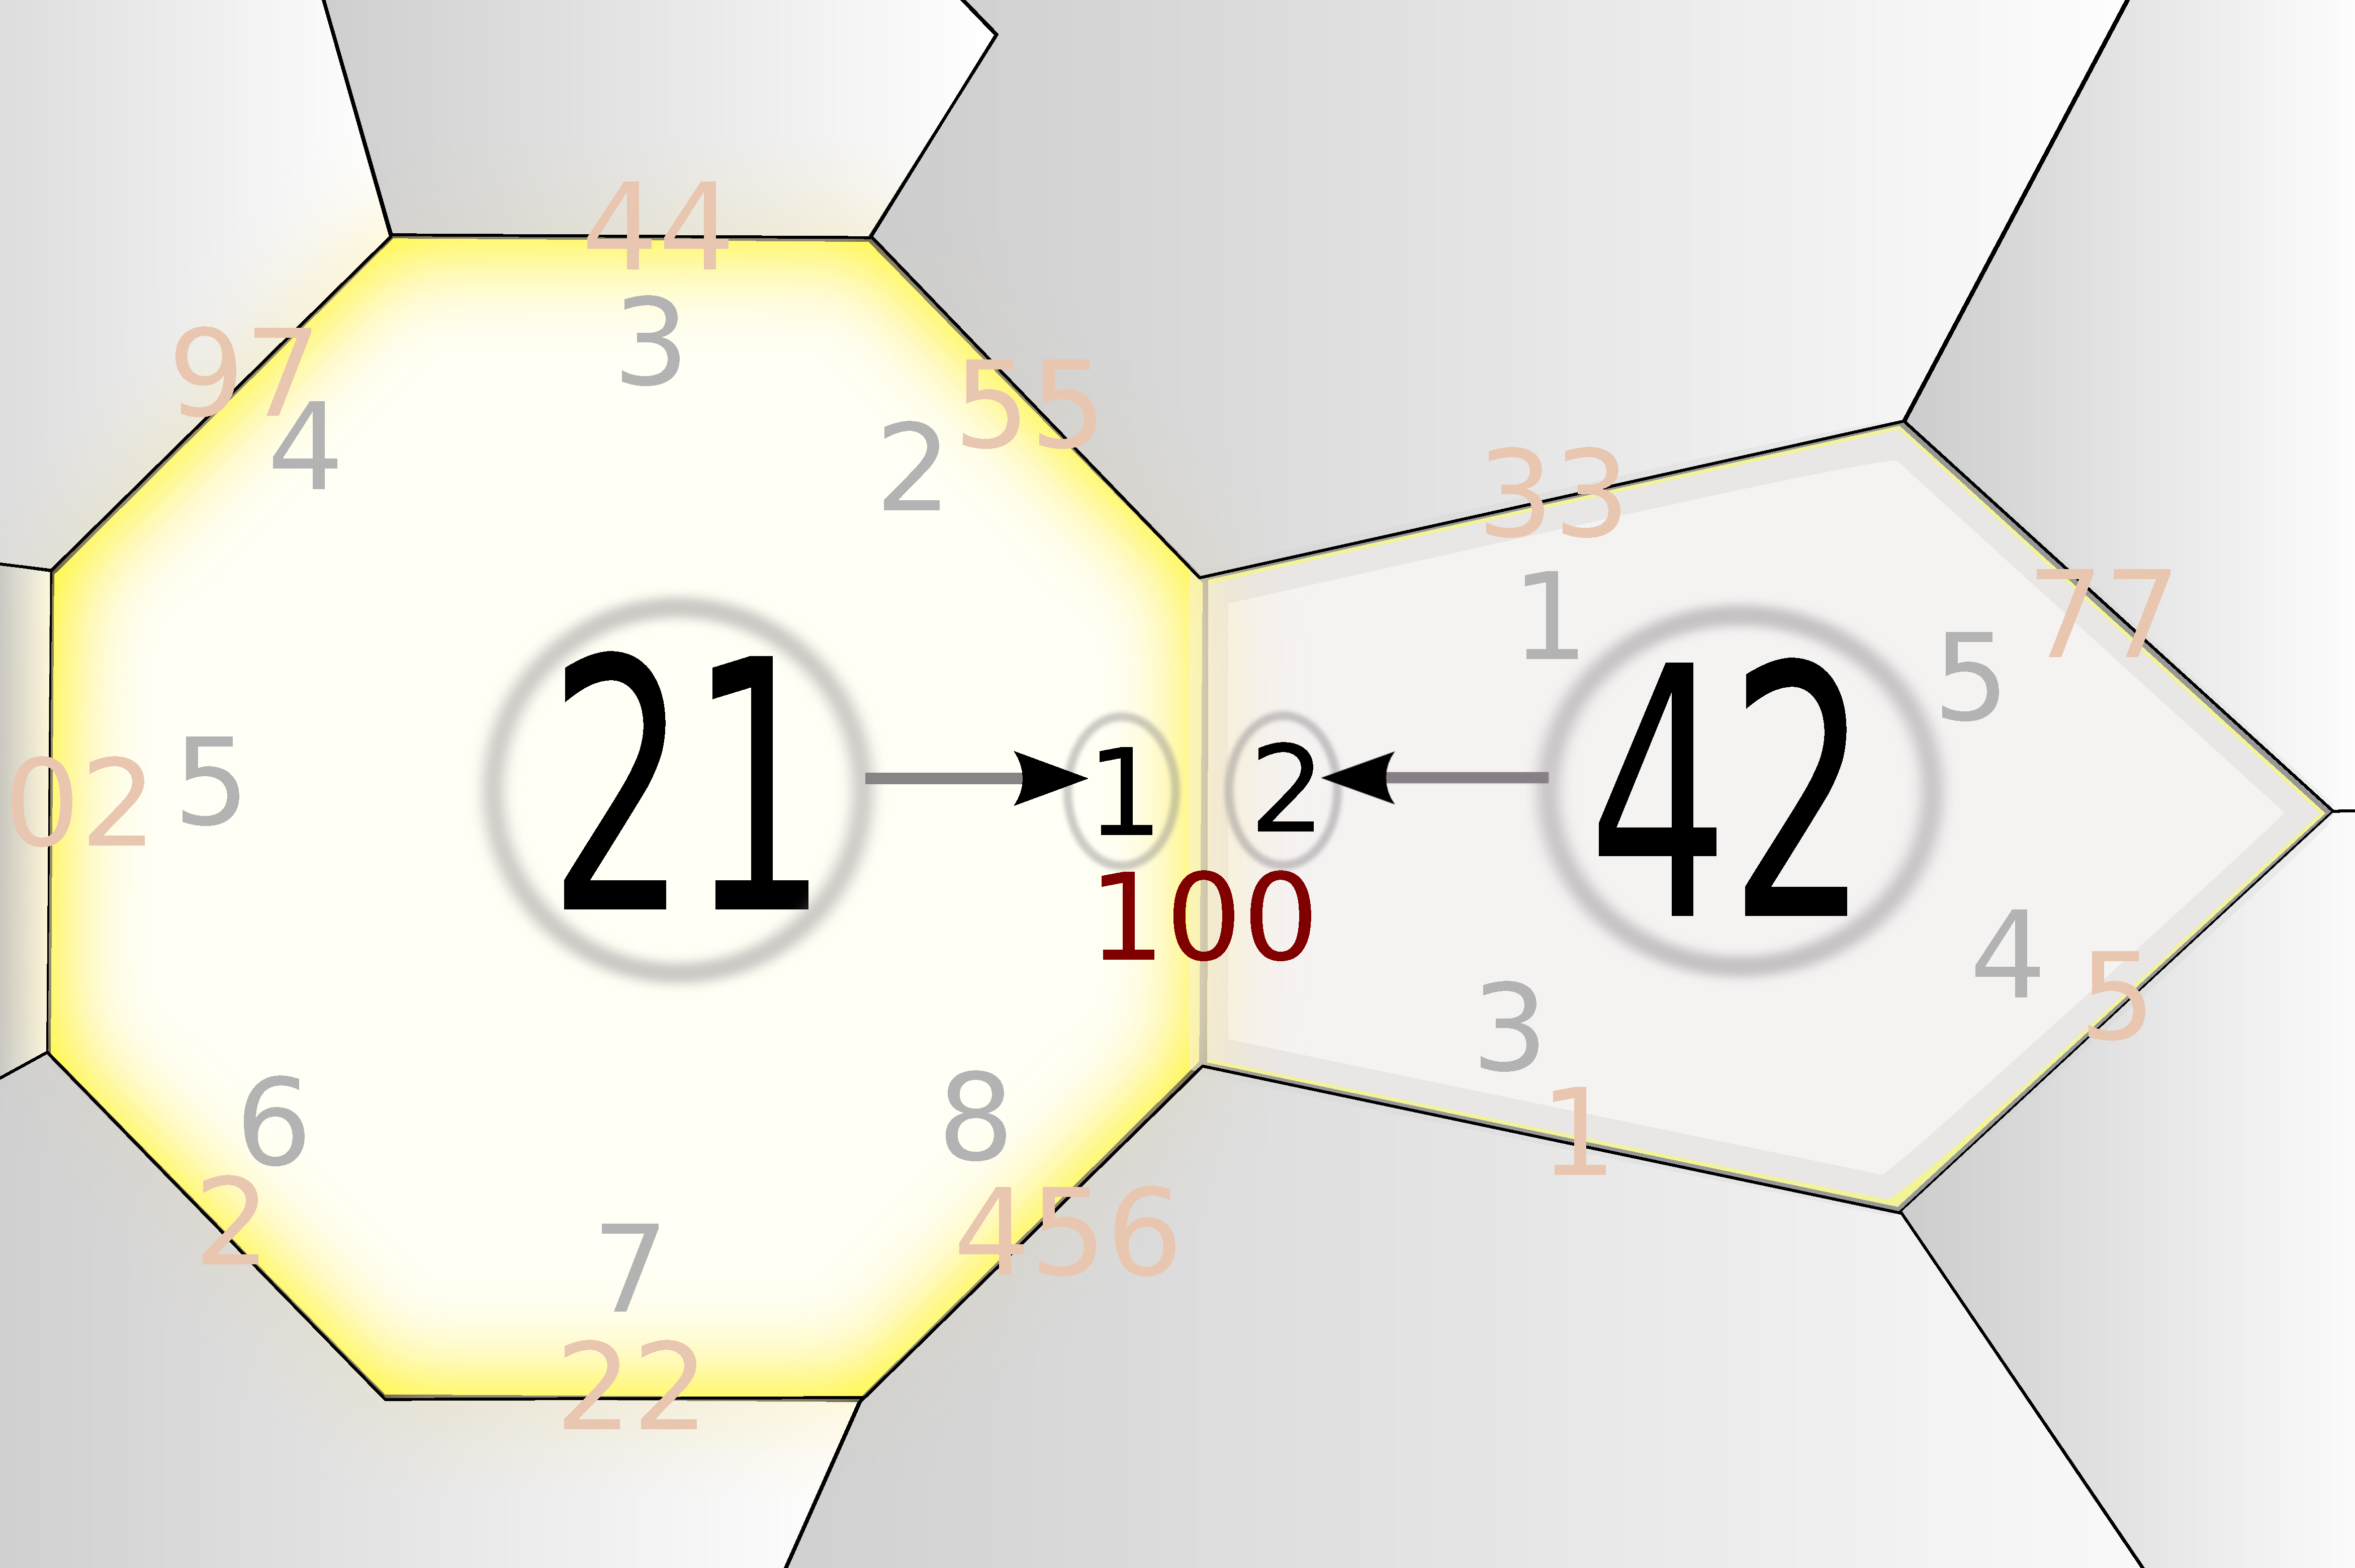
\includegraphics[width=6cm, height=4cm]{img/two_fes_nbsideincls.pdf}}}
      }
  \end{columns}
  \begin{itemize}[<+->]
    \item The \emph{\textbf{finite element inclusions}} of a non-boundary side are the couple of finite elements which include the side,
      each paired with the side face of the side in the including element.
    \item For any non-boundary side, represents the two \emph{\textbf{local representations}} of the side as it occurs in finite elements.
  \end{itemize}
\end{frame}

\subsubsection{Summing Up: Initial Mesh Contract}

\begin{frame}
  \frametitle{Summing Up Mesh Concepts: Initial Mesh Contract}
  \begin{itemize}[<+->]
    \item We can already determine some of the requirements for our abstract mesh contract.
    \item Types \\
      $FENum, NBSideNum, OShape, SideFace = \mathbb{N}$.\\
      $NBSideInclusions = (FENum \times SideFace) \times (FENum \times SideFace)$.
    \item Then the mesh must provide the following functions (incomplete):
      \begin{itemize}[<+->]
        \item \textcolor{blue}{num\_fes}: $() \rightarrow \mathbb{N}$
        \item \textcolor{blue}{num\_nb\_sides:} $() \rightarrow \mathbb{N}$
        \item \textcolor{blue}{num\_oriented\_element\_shapes}: $() \rightarrow \mathbb{N}$
        \item \textcolor{blue}{oriented\_shape\_for\_fe}:  $FENum \rightarrow OShape$
        \item \textcolor{blue}{num\_side\_faces\_for\_shape}: $OShape \rightarrow \mathbb{N}$
        \item \textcolor{blue}{fe\_inclusions\_of\_nb\_side}: $NBSideNum \rightarrow NBSideInclusions $
        \item \textcolor{blue}{nb\_side\_num\_for\_fe\_side}: $FENum \times SideFace \rightarrow NBSideNum$
      \end{itemize}
  \end{itemize}
\end{frame}

\subsection{Approximation space}

\subsubsection{Shape Functions}

\begin{frame}
  \frametitle{WG Shape Functions}
  \begin{itemize}[<+->]
    \item The WG approximation space consists of piecewise polynomials on mesh element interiors and non-boundary sides,
      satisfying degree constraints, and which are 0 on mesh boundary sides.
    \item Interiors and sides may have distinct degree constraints as groups, each limited either by max monomial degree or max variable degree.
    \item As a building block for our basis, we'll define a \emph{\textbf{shape function}} to be a function which is a monomial on one face
      (interior or side) pre-composed with a translation function providing a face-specific origin, which satisfies the appropriate
      degree constraint for the face.
    \item Such shape functions can be chosen to equal any untranslated polynomials of the same degree constraint on their supporting faces,
      which implies that these shape functions taken together \emph{\textbf{span the WG approximation space}}. 
  \end{itemize}
\end{frame}


\subsubsection{Face-Local Origins}

\begin{frame}
  \frametitle{Face-Local Origins for Shape Functions}
  \begin{itemize}[<+->]
    \item Use of face-local coordinates allows many computations involving shape functions to be done only once per oriented shape
      instead of once per finite element, which is crucial for computational efficiency.
    \item To achieve this, face-local origins must be chosen carefully.
    \item A face's local origin should \emph{not} be chosen based on the face's inclusion in a specific element, which would preclude doing
          calculations on oriented shapes as proxies for multiple finite elements.
    \item A side's local origin should \emph{not} be chosen based on the side's membership in an oriented shape, because this representation
      is not unique.
    \item Local origins \emph{\textbf{should}} be based on some \emph{\textbf{translation-independent}}, \emph{\textbf{intrinsic}} geometric
      property of the face. Good choices are the \textbf{centroid}, or the \textbf{vertex of minimum coordinates}.
  \end{itemize}
\end{frame}

\begin{frame}
  \frametitle{Face-Local Origins for Shape Functions (Contd)}
  \begin{columns}
    \column{.50\textwidth}
      \frame{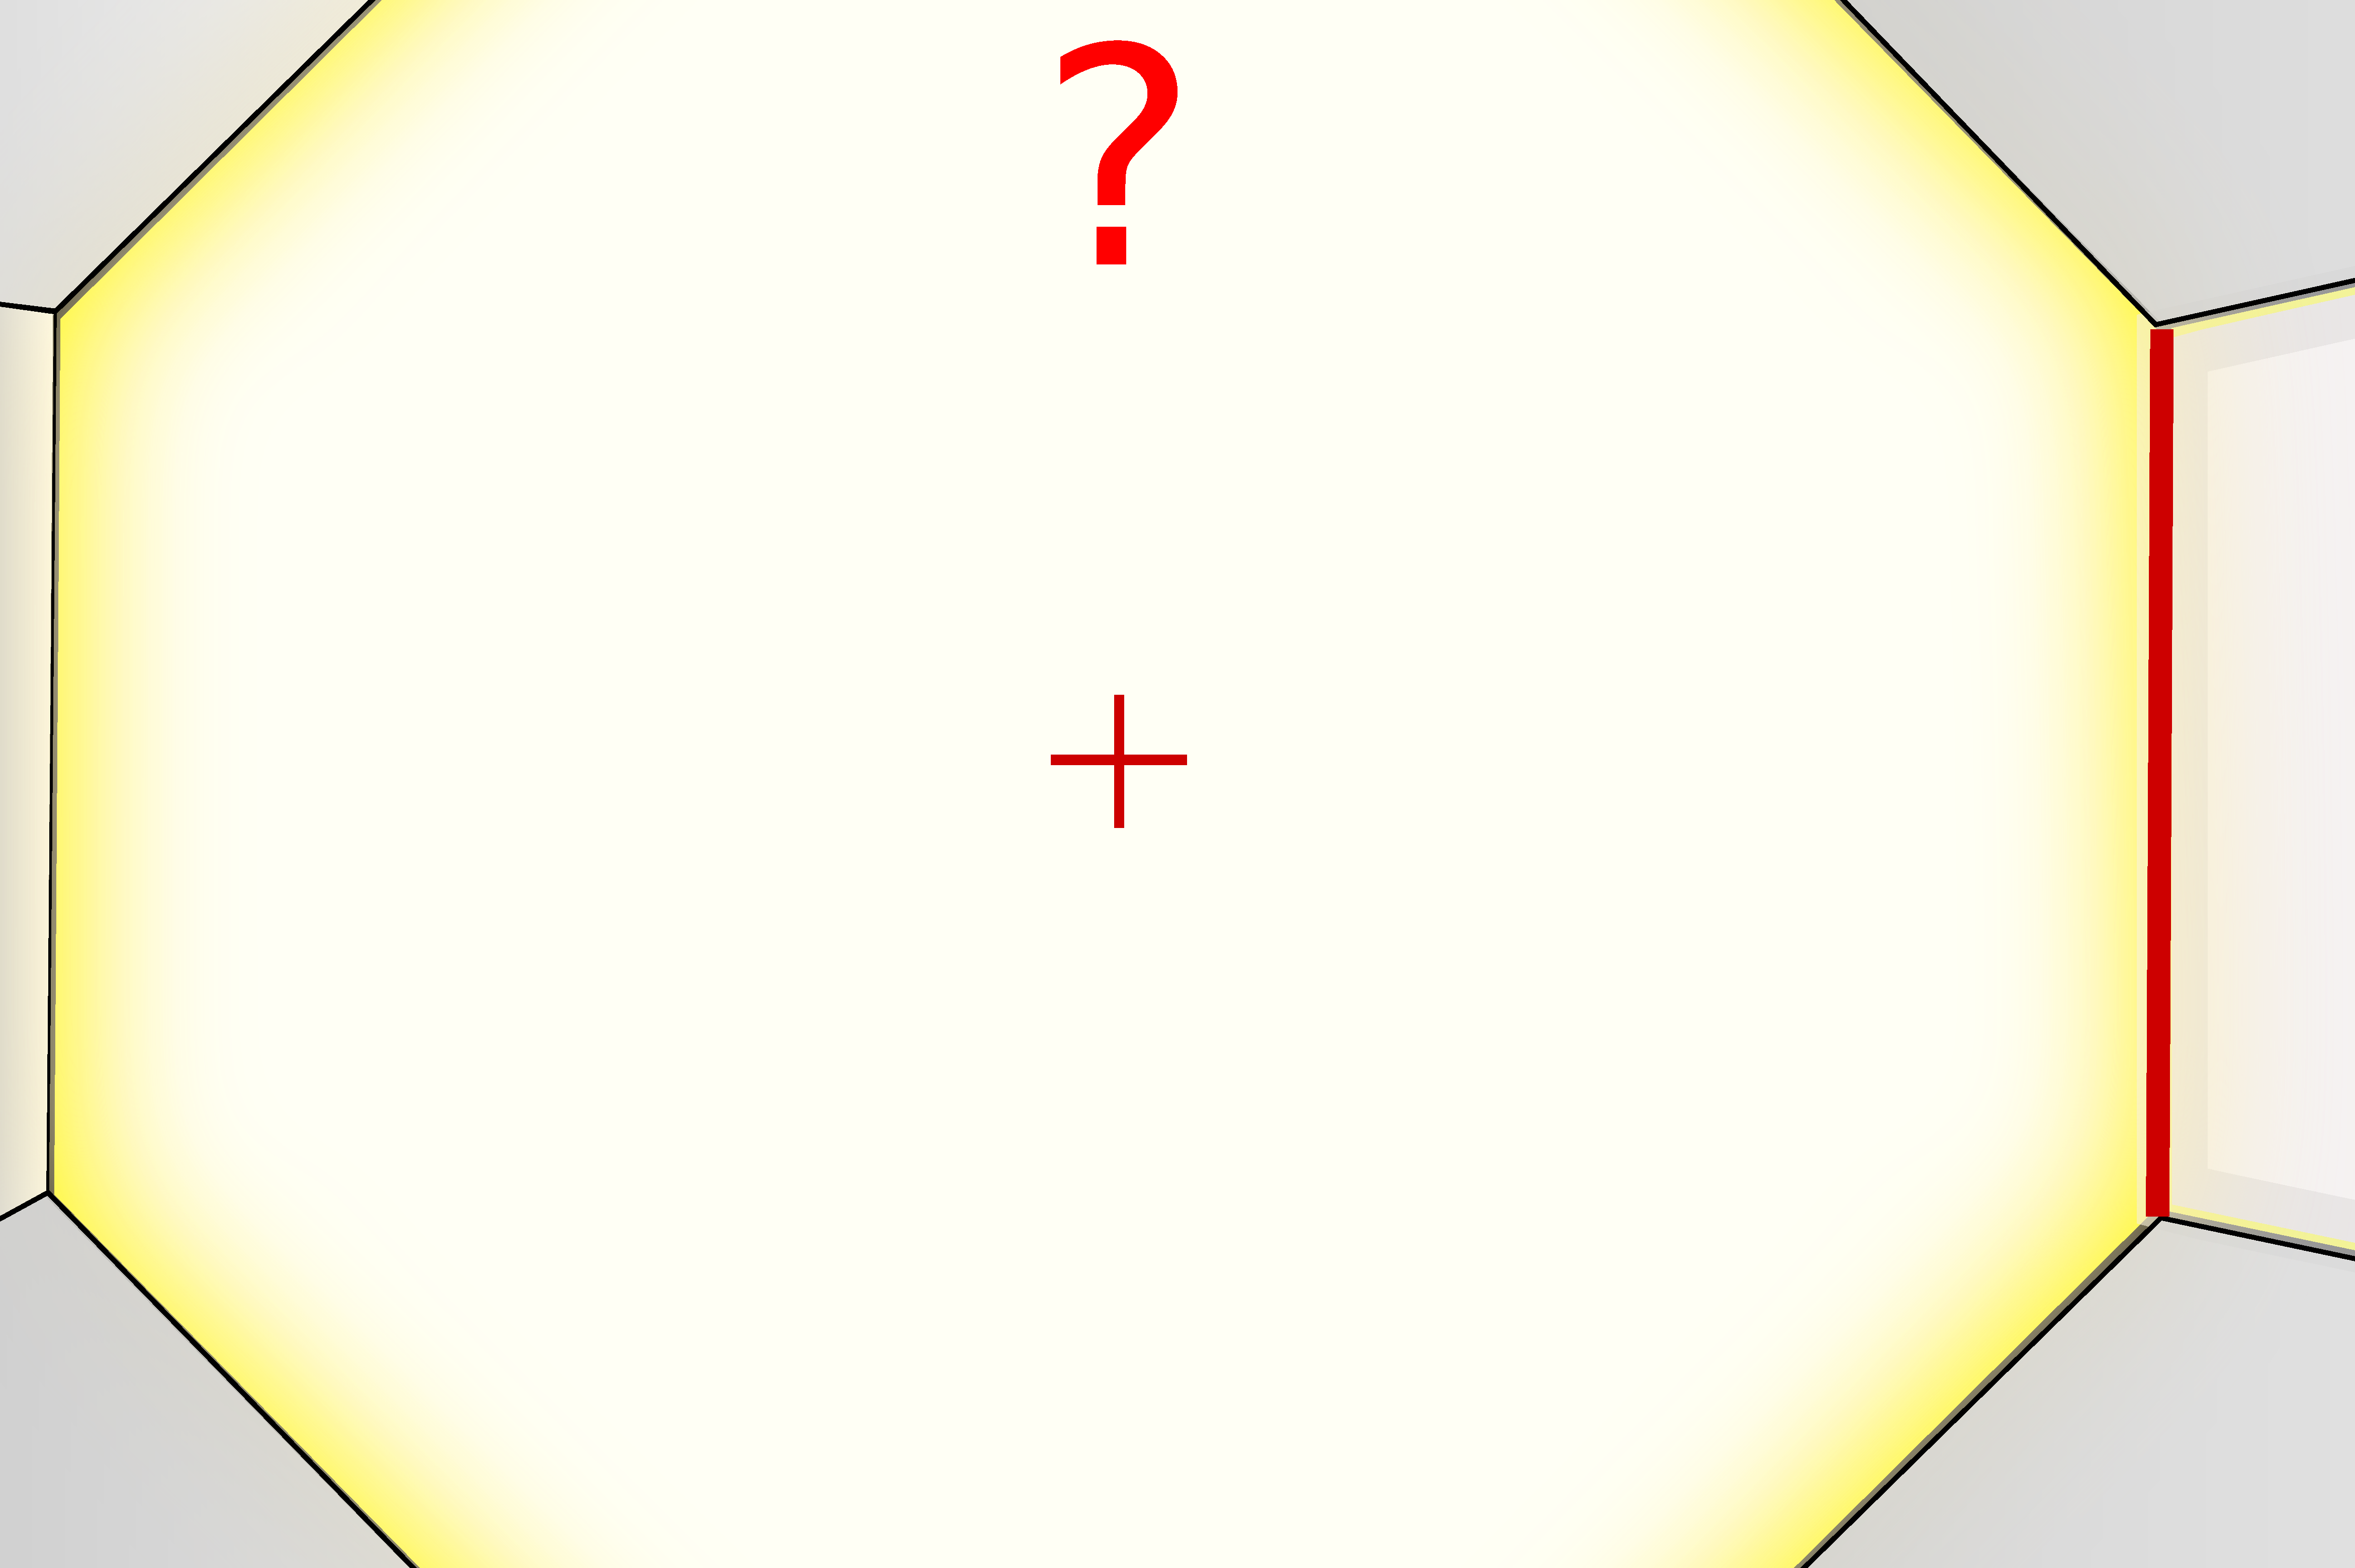
\includegraphics[width=6cm, height=4cm]{img/two_fes_bad_side_origin_1.pdf}}
    \column{.50\textwidth}
      \frame{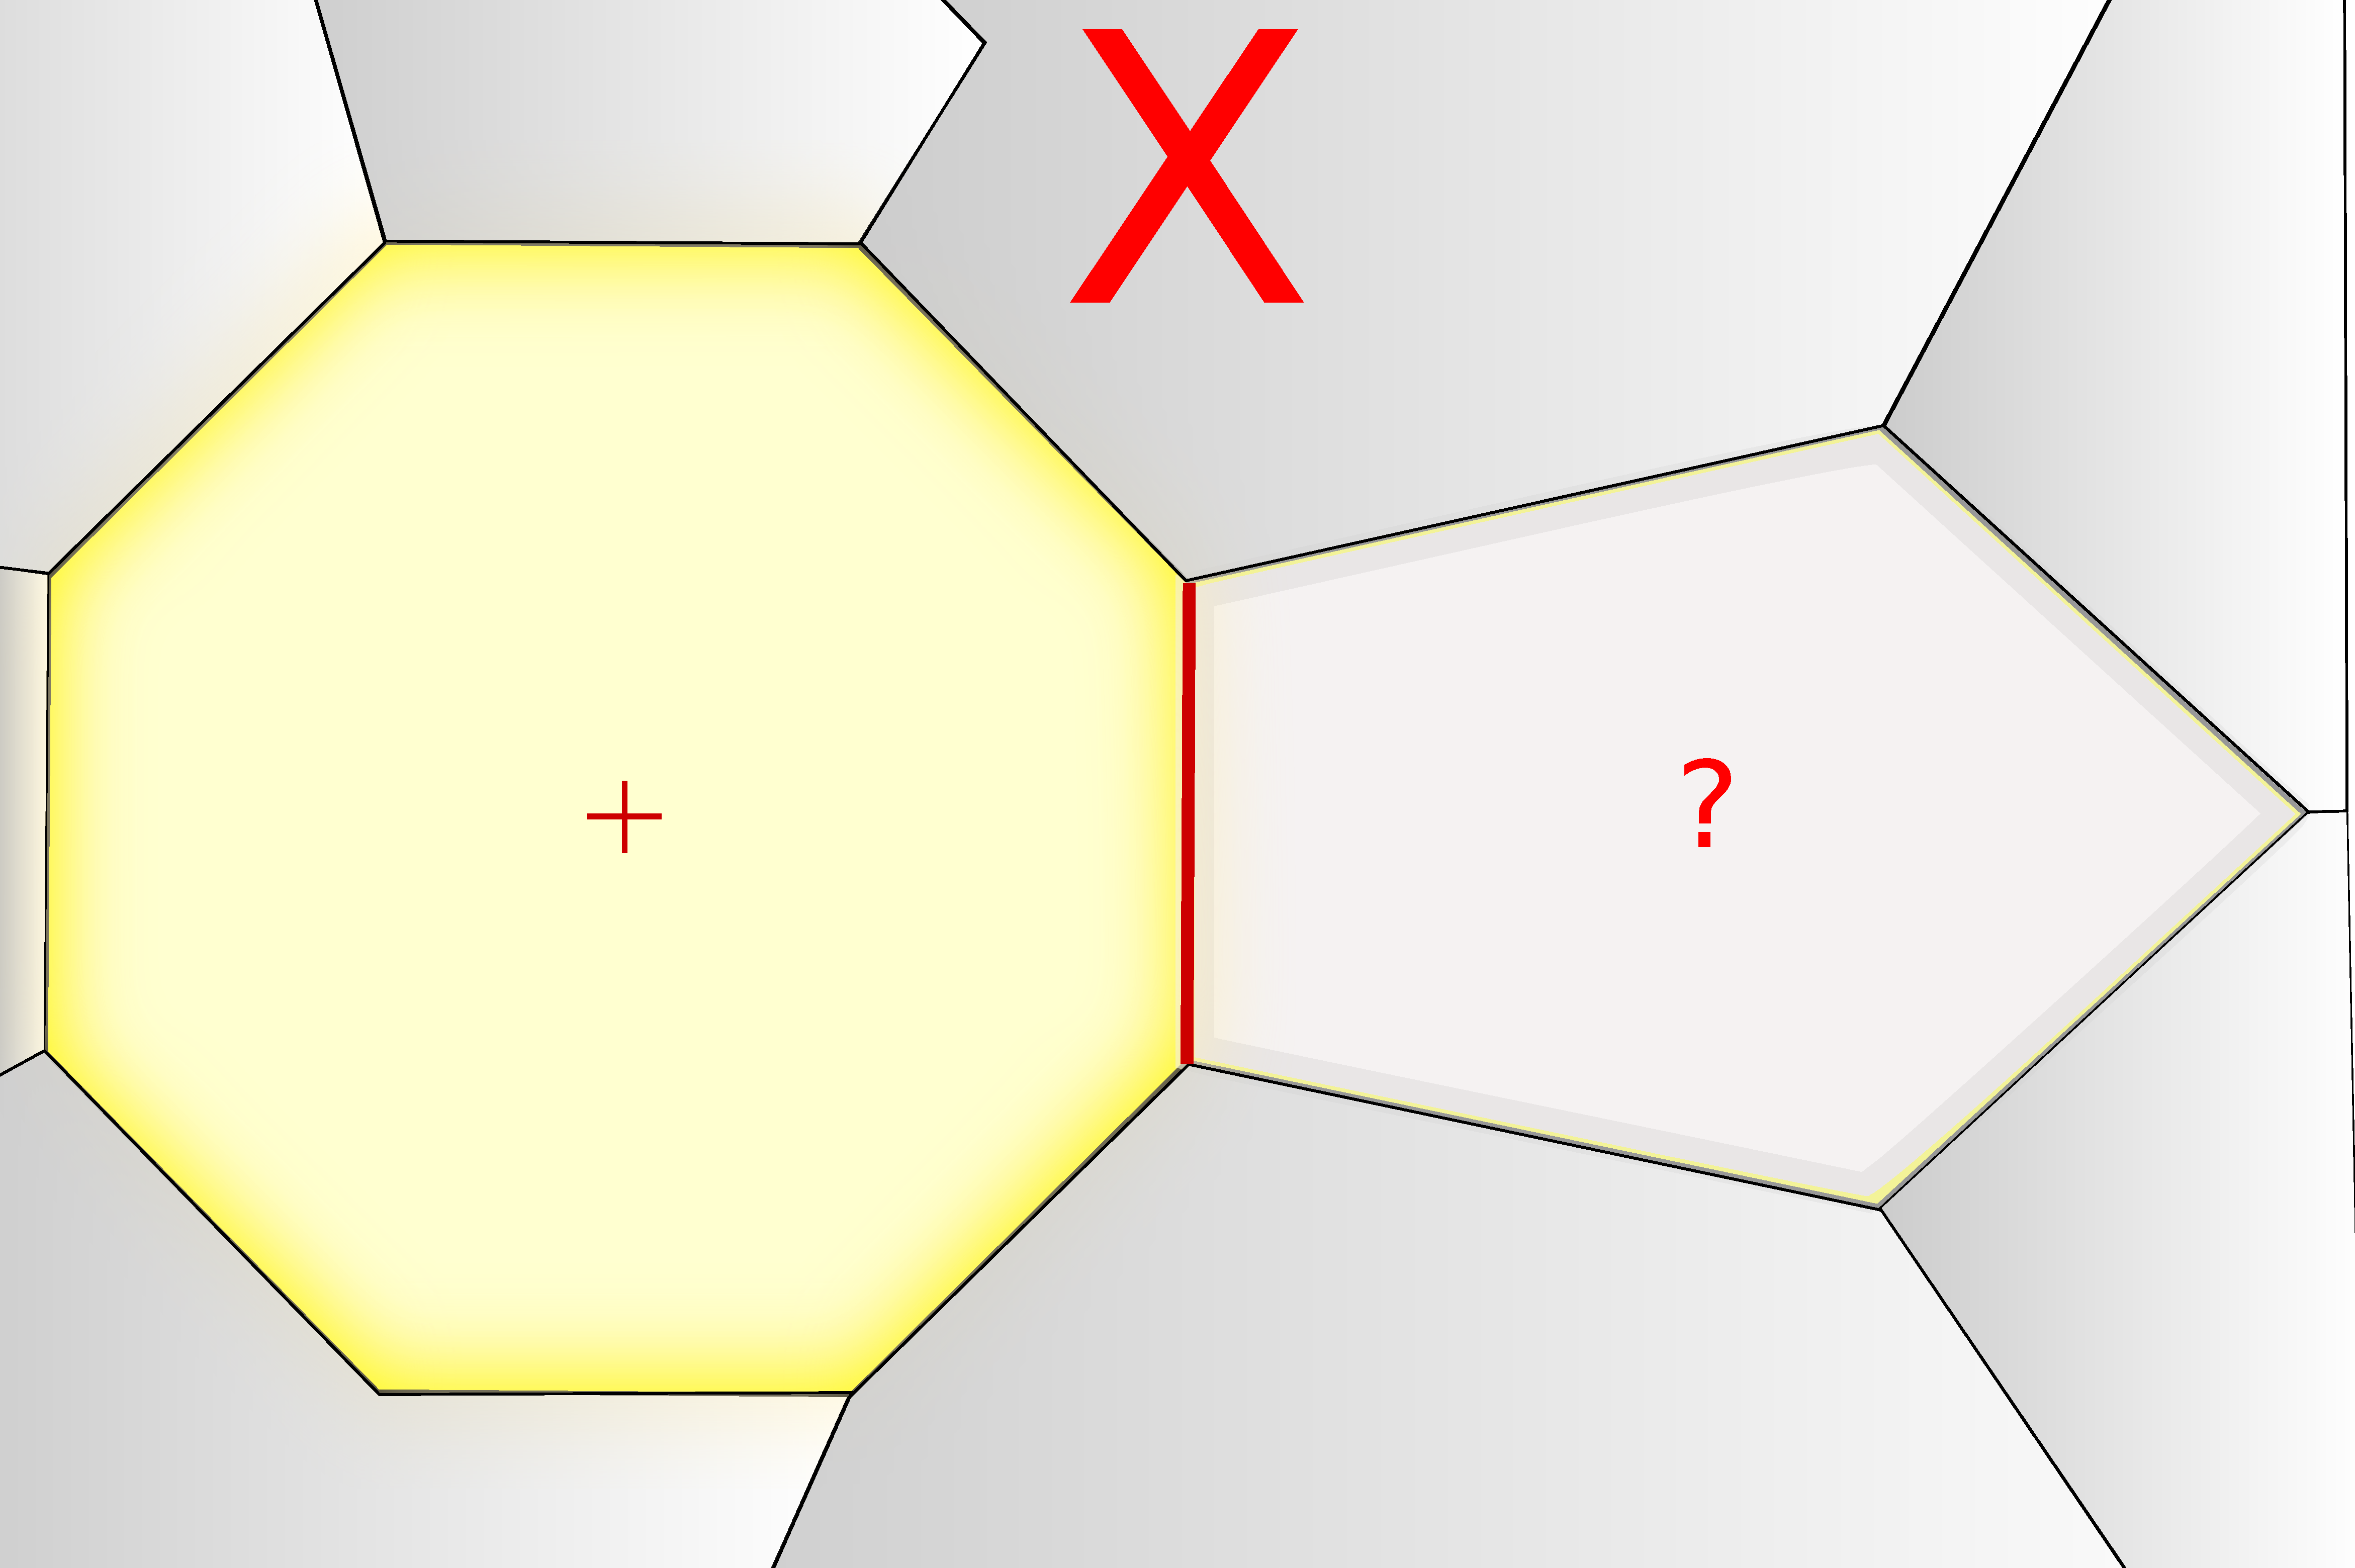
\includegraphics[width=6cm, height=4cm]{img/two_fes_bad_side_origin_2.pdf}}
  \end{columns}
  \begin{itemize}[<+->]
    \item On the left, it is tempting to choose a common origin for the sides and interior of the element, to make calculations easier.
    \item This choice would be difficult to apply consistently, however. A calculation on the right hand element must also use this origin
      for its left side, even if specific elements are not in context such as for calculations on the oriented shape for the right element.
      Rules could be applied in special meshes to achieve this, but they would be ``fragile'' because of the number of assumptions required.
  \end{itemize}
\end{frame}

\subsubsection{Shape Function Independence}

\begin{frame}
  \frametitle{Shape Function Independence}
  \begin{columns}
    \column{.50\textwidth}
      \frame{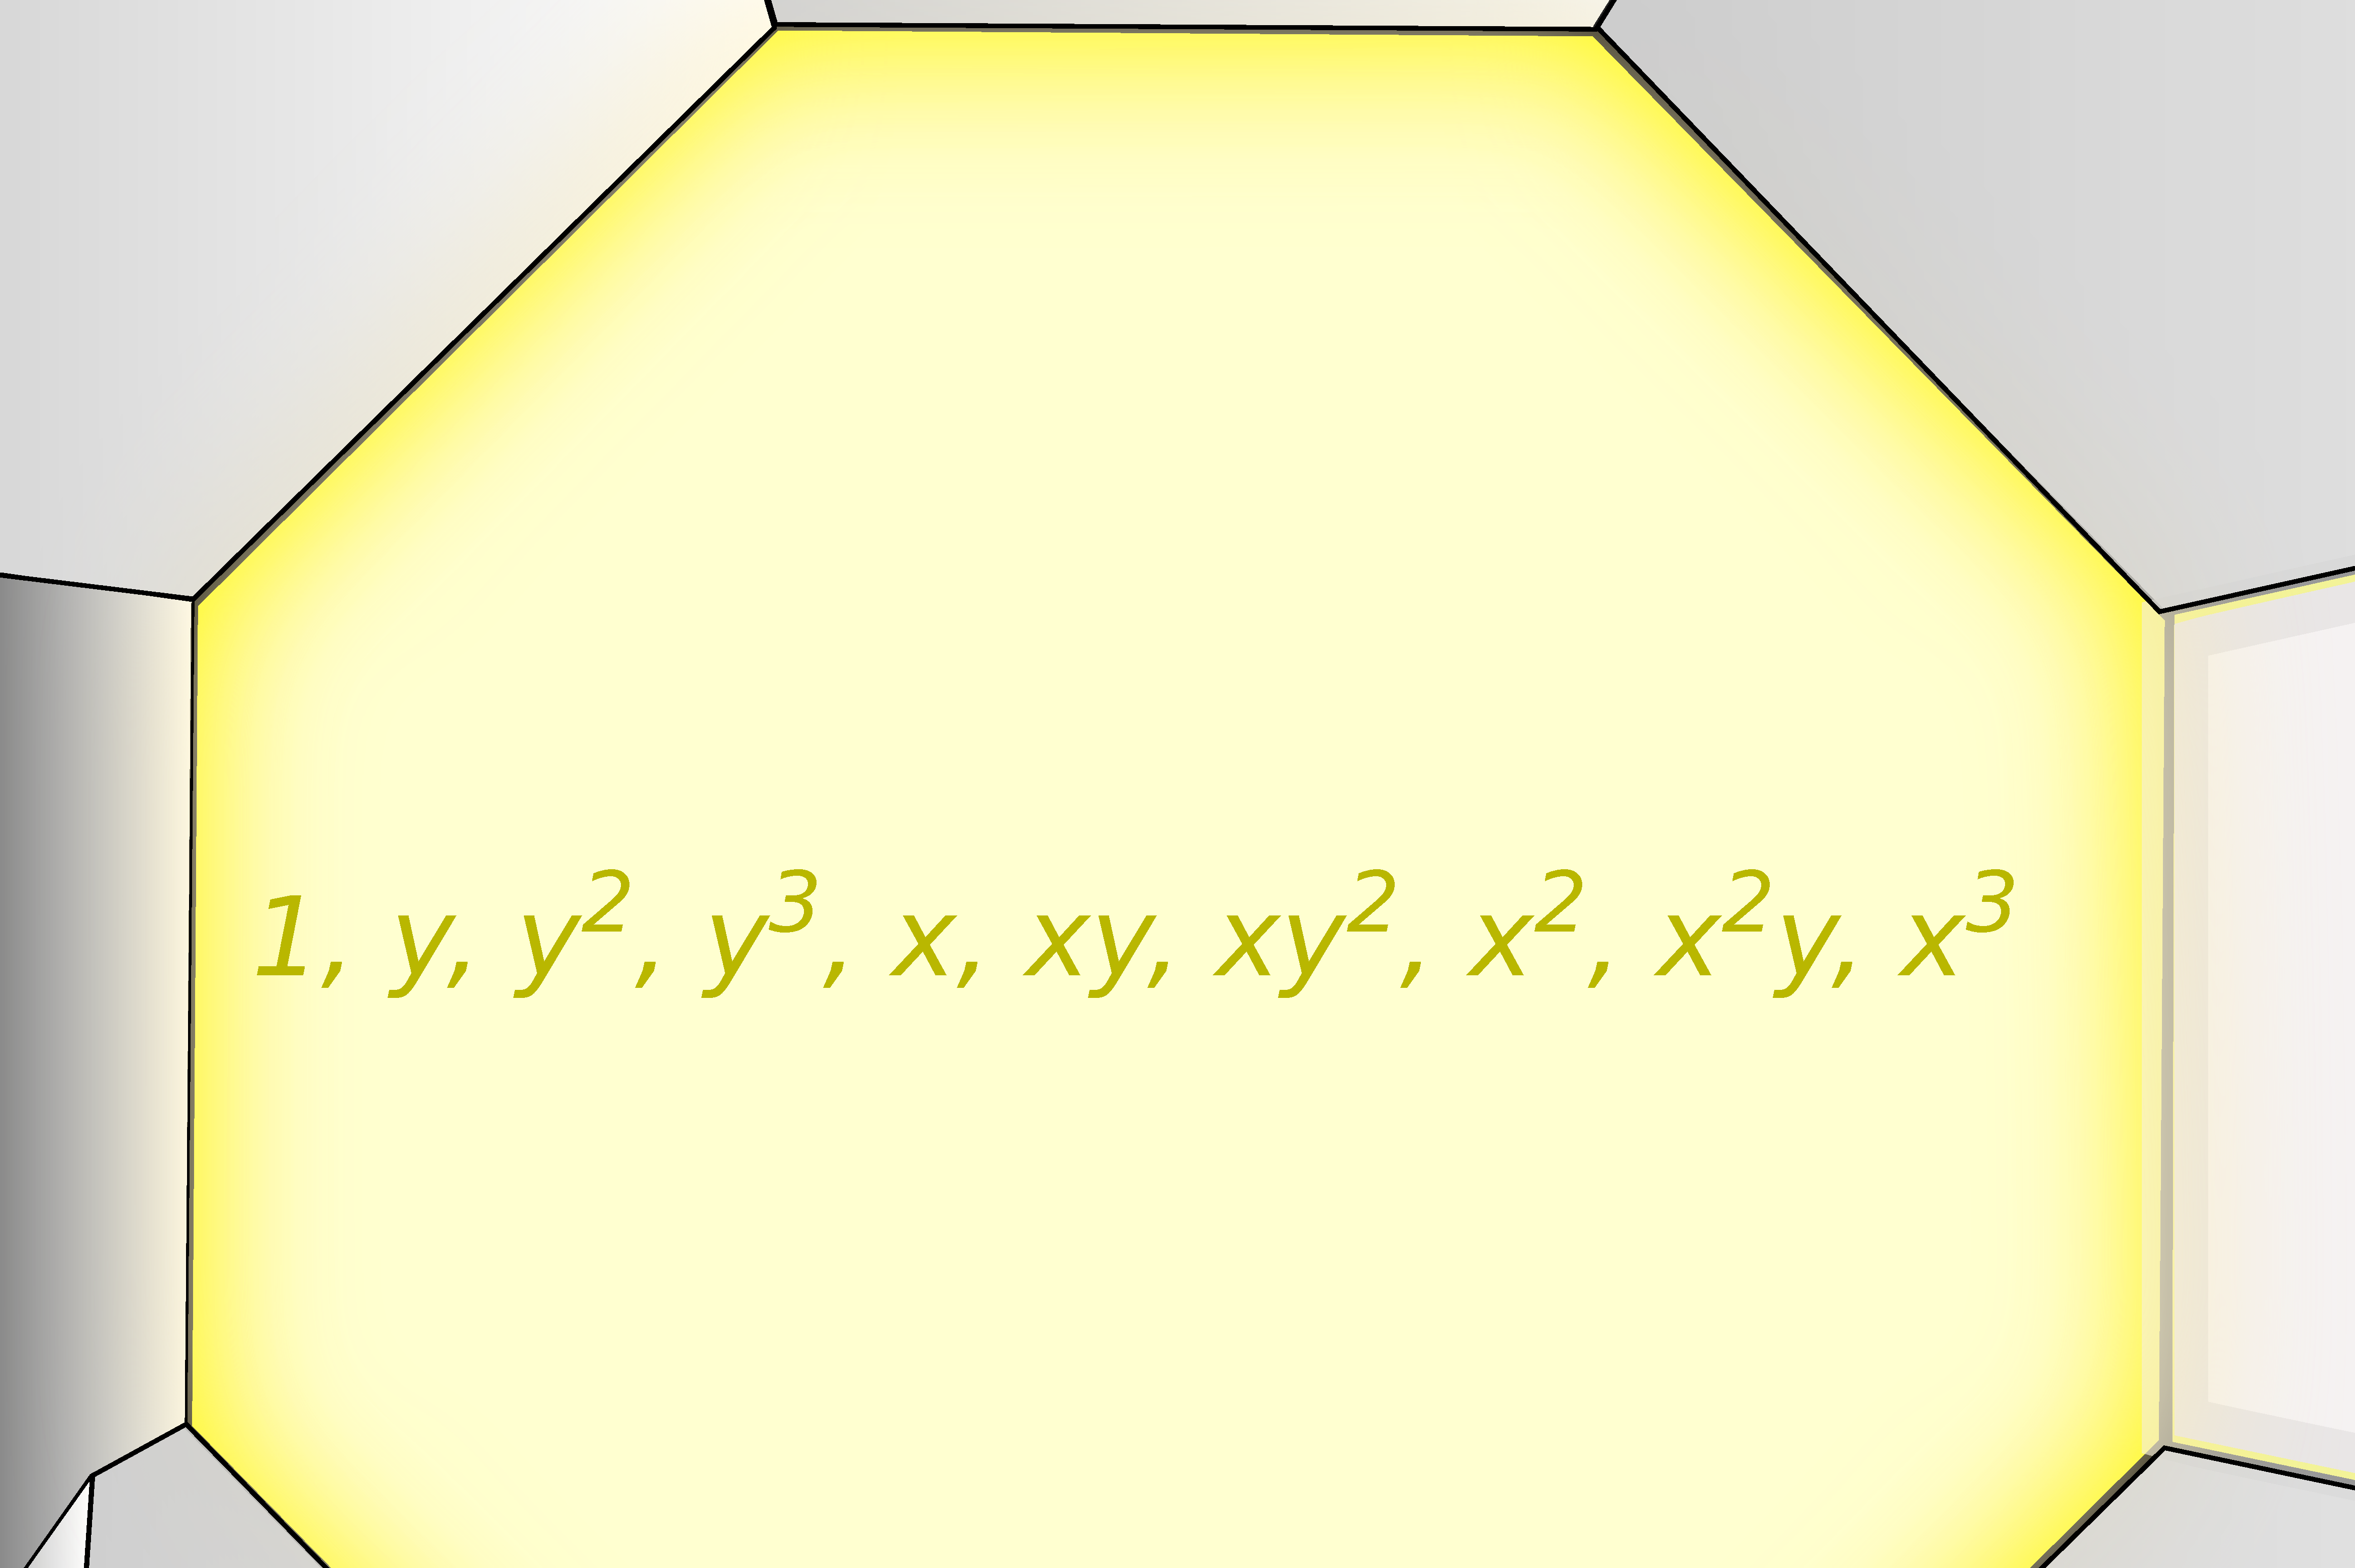
\includegraphics[width=6cm, height=4cm]{img/fe_shapefun_int_mons.pdf}}
    \column{.50\textwidth}
      \pause
      \begin{itemize}[<+->]
        \item Interior supported shape functions are linearly independent by the fundamental theorem of algebra.
          Otherwise we would have a polynomial with a non-zero coefficient and an infinite number of roots.
      \end{itemize}
  \end{columns}
  \uncover<+-> {
    \begin{columns}
    \column{.50\textwidth}
    \frame{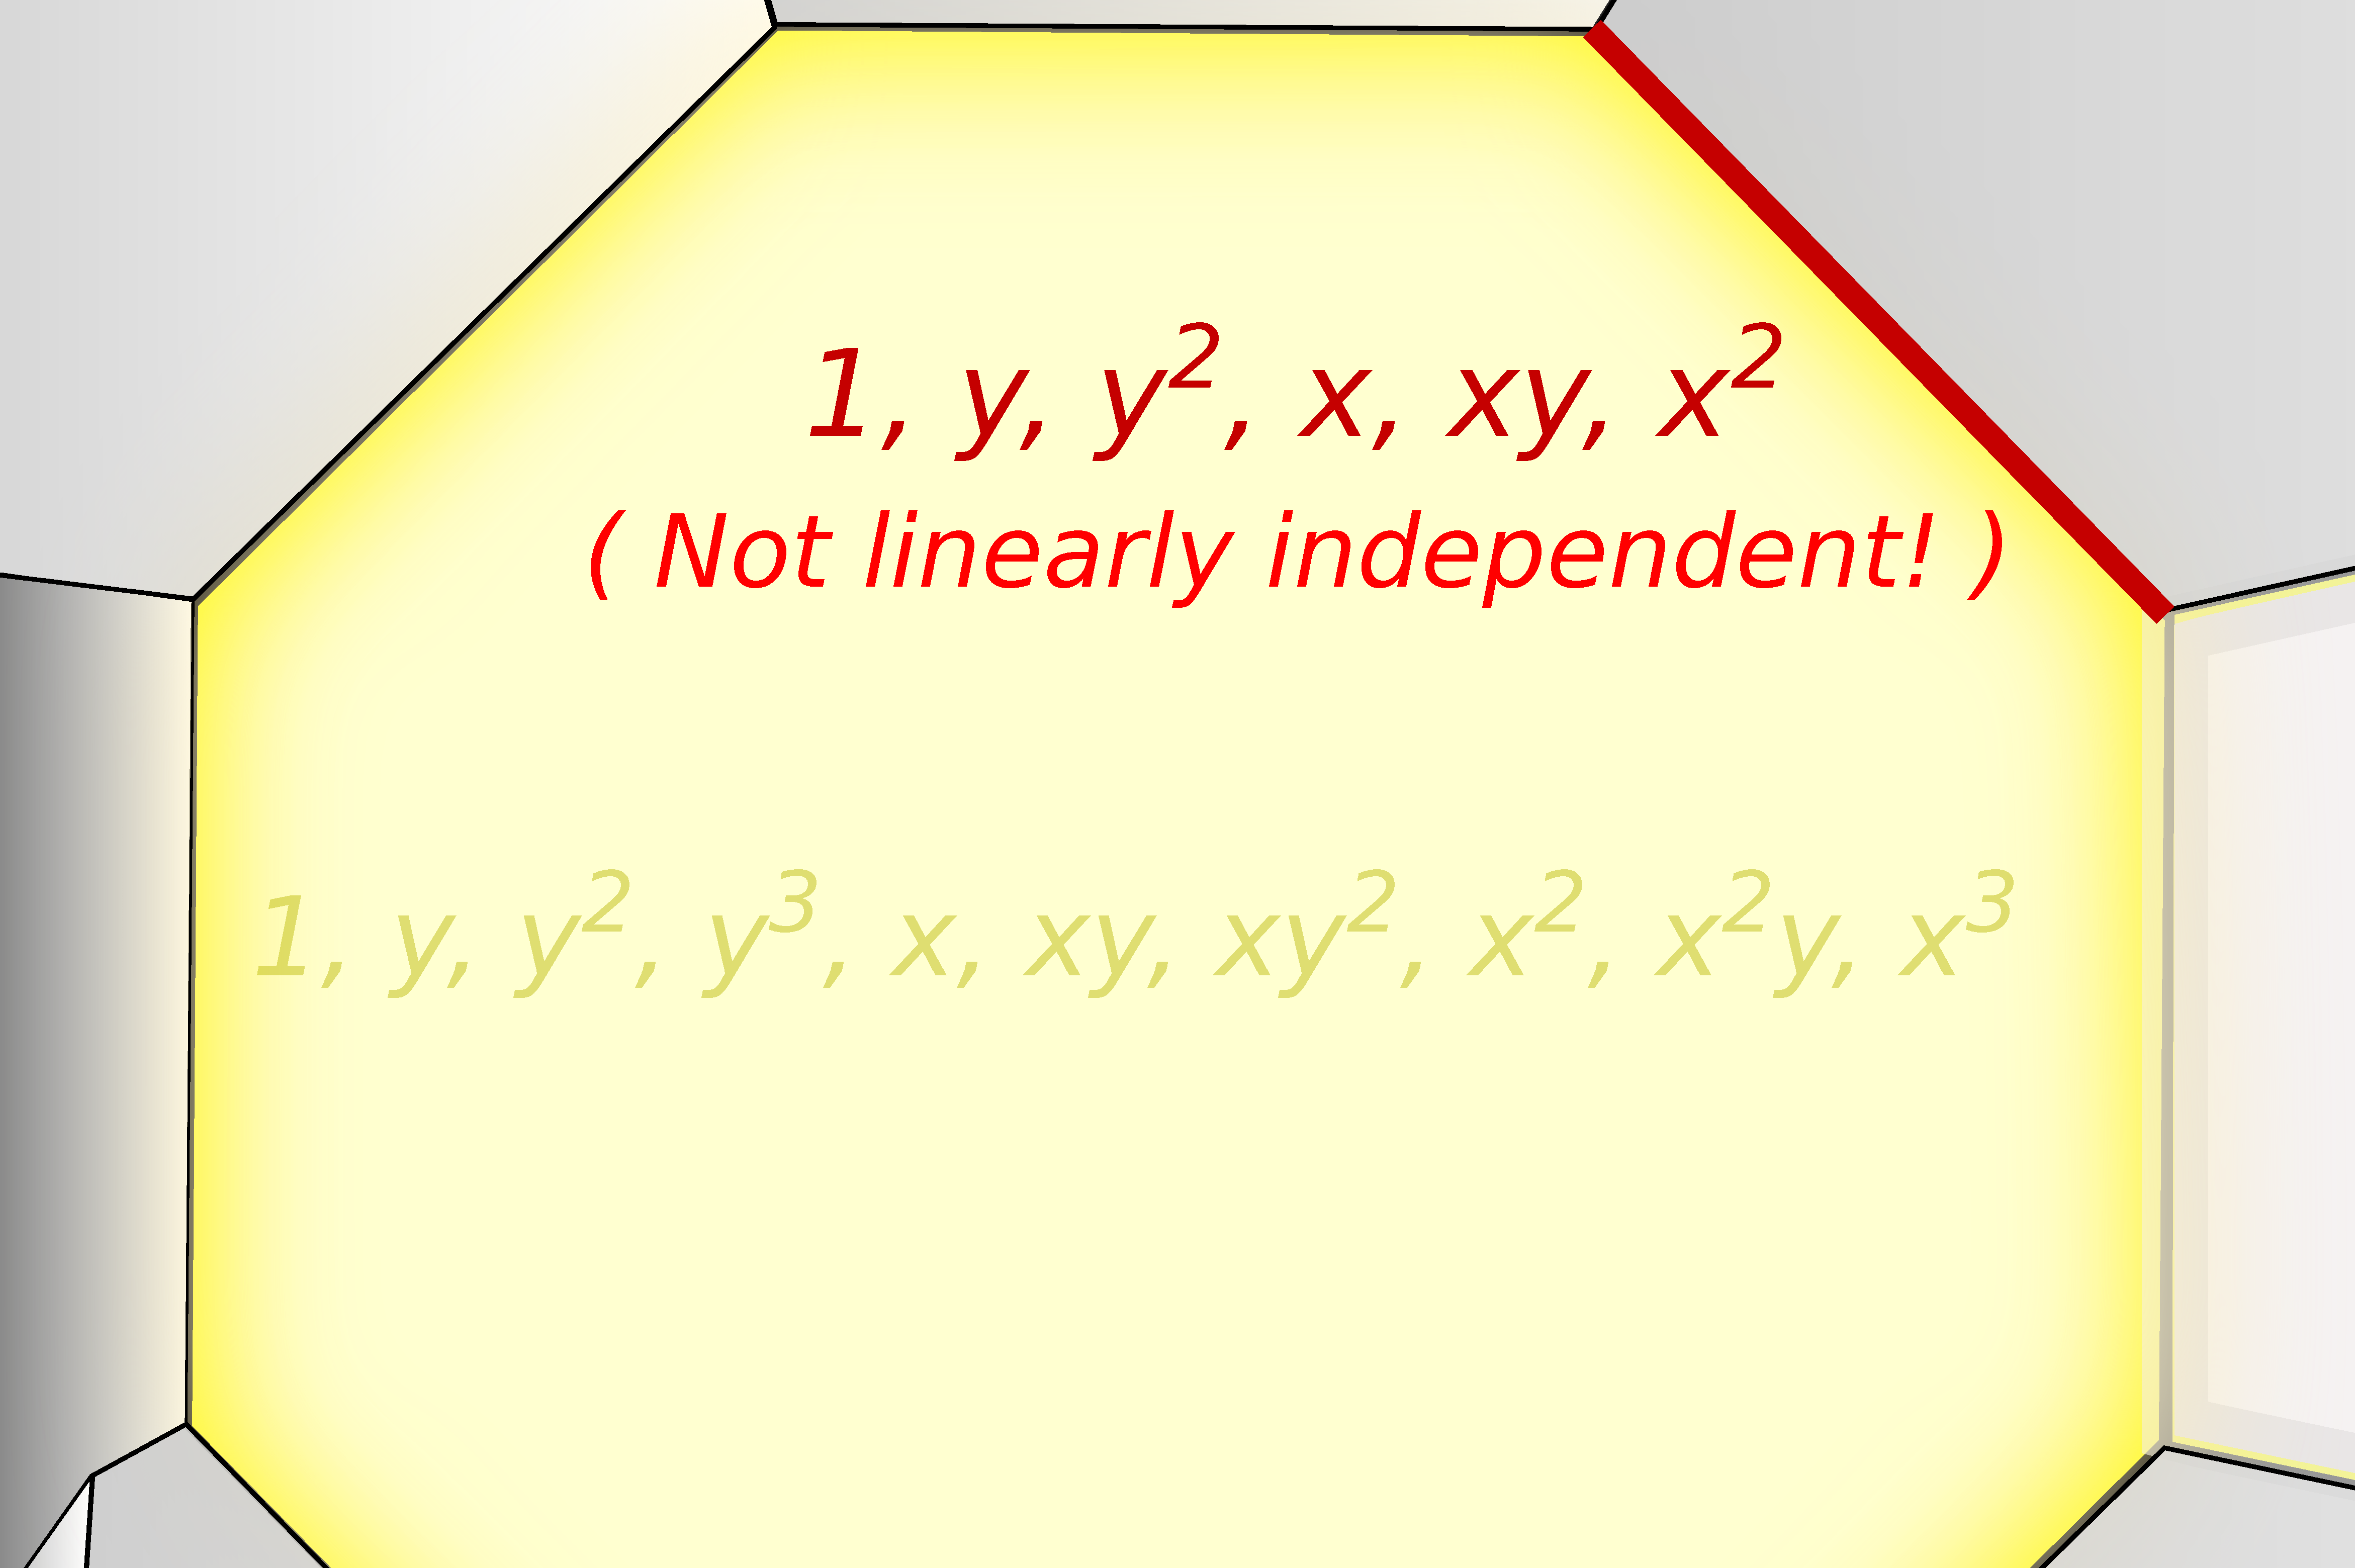
\includegraphics[trim=30pc 40pc 0cm 0cm, clip=true, width=6cm, height=3.4cm]{img/fe_shapefun_side_mons_int_greyed.pdf}}
    \column{.50\textwidth}
      \begin{itemize}[<+->]
        \item However the full set of side supported shape functions are \emph{\textbf{linearly dependent}}. E.g. $y=-x$ for all $(x,y)$ on the side pictured,
          so that $y^2=x^2$, $x y = -x^2$, etc.,  on the side.
      \end{itemize}
    \end{columns}
  }
\end{frame}

\subsubsection{Side Dependent Dimension}

\begin{frame}
  \frametitle{Side Dependent Dimension}
  \begin{itemize}[<+->]
  \item The subset of shape functions supported on a side which are linearly independent depends on the side's orientation.
  \item Each side has at least one \emph{\textbf{dependent dimension}}, which is a space dimension which can be written as an affine
      function of the others on the side, as expressed in the side's local coordinate system.
  \end{itemize}
  \uncover<+-> {
    \begin{block}{Existence of Dependent Dimension for a Side}
      We take as given that a side is a translated subset of a subspace $S$ of dimension $d-1$ of $\mathbb{R}^d$. Then $S$ is the solution
      of a single linear equation, $S = \left\{(x_1,\dots,x_d): \sum_{i} a_i x_i = 0\right\}, \text{where some } a_j \ne 0$,
        so that $x_j$ is a linear combination of the other $x_i$ on $S$. This holds for coordinates relative to an origin within $S$.
        If the side's origin is outside the side, then recasting to that origin yields an affine function.
    \end{block}
  }
\end{frame}

\begin{frame}
  \frametitle{Side Dependent Dimensions Illustrated}
    \frame{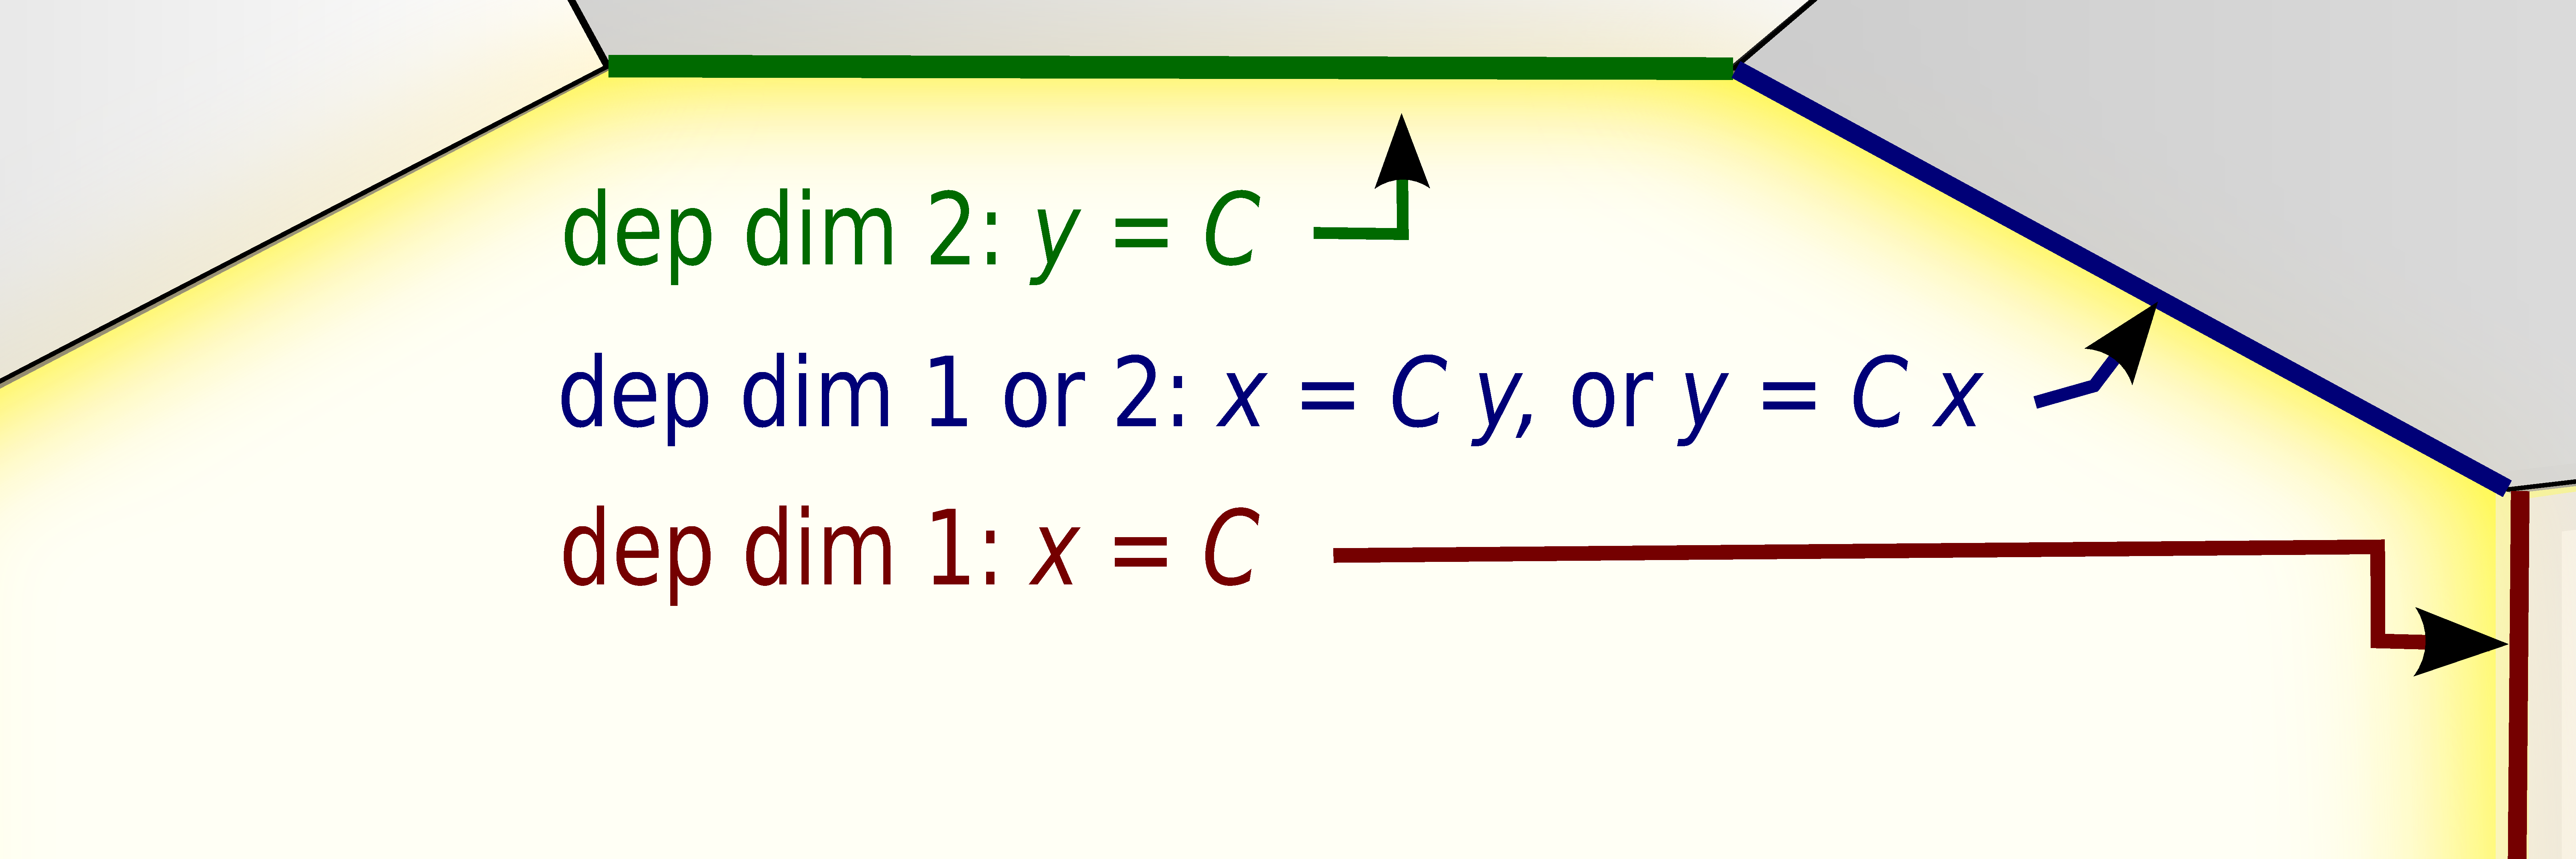
\includegraphics[width=12cm, height=4cm]{img/side_dep_dims_2d.pdf}}
    \begin{itemize}[<+->]
      \item Dependent dimensions must be chosen by the mesh for \emph{each} side, so the basis can choose shape functions to support on the sides.
        Commonly a side has multiple dependent dimensions, from which the mesh must choose one.
      \item Choice should be based on intrinsic geometric properties of the side, not its representation in finite elements
        (which precludes oshape ops) or in oriented shapes (representation not unique).
    \end{itemize}
\end{frame}


\begin{frame}
  \frametitle{Side Dependent Dimension -- Contd}
  \begin{itemize}[<+->]
    \item To form a linearly independent set of shape functions supported on a side, we will \emph{\textbf{omit the shape functions
      having any non-zero power of the dependent dimension variable}}.
    \item The reduced set of shape functions spans the same space as the full set, because with dependent dimension of $j$,
      any monomial of the full set can be expressed as
       $$x_1^{k_1} \dots x_j^{k_j} \dots x_d^{k_d}
           \;\; = \;\; x_1^{k_1} \dots (a_0 + \sum_{i \ne j} a_i x_{i})^{k_j} \dots x_d^{k_d}\text{,}$$
      which expands to a polynomial which is free of $x_j$. Additionally, the right side's maximum monomial degree will not exceed
      that of the left.  For constraints on the maximum variable degree, if $a_i = 0$ for $i \ge 1$,
      as is the case with rectangle meshes, then we again have the right hand side satisfying any max variable degree constraint
      that the left side does. In either case, the right hand side is a linear combination of monomials in the reduced set, proving
      that our reduced set spans the full space.
    \item That they are linearly independent needs to be proved (TODO).
  \end{itemize}
\end{frame}

\subsection{Variational Bilinear Form}

\subsubsection{Practicality of Computation}

\begin{frame}
  \frametitle{Variational Bilinear Form - Practicality}
  $$\spot<1->{\mathfrak{a}}(u_h,v) = (f,v)\quad\quad \forall{v} \in V_{h0}$$
  \begin{itemize}[<+->]
    \item Some additional requirements on the vbf are necessary for computations to be feasible at even moderate scale.
    \item For example for $k=3$ and a 50x50 mesh, there are already 39,700 basis elements, and \emph{1,576,090,000} 
      \emph{interactions} between elements. 
    \item The majority of these interactions will yield $0$ vbf value, but we need to avoid computing as many as possible.
    \item We'll use two additional requirements on the vbf to eliminate many unnecessary calculations:
        \begin{itemize}[<+->]
          \item \emph{\textbf{Element summability}} and associated \emph{\textbf{locality}} property, allowing element-wise operations and
            forbidding ``action at a distance''
          \item a \emph{\textbf{translation invariance}} property, allowing calculations to be done on a general oriented shape in place of
            calculations on individual finite elements of the shape
        \end{itemize}
    \item Requirements are aligned with general spirit of FEM's.
  \end{itemize}
\end{frame}

\subsubsection{Element Summability}

\begin{frame}
  \frametitle{Variational Bilinear Form -- Element Summability}
  \begin{block}{Element Summability}
    The vbf is the sum of contributions of a fixed \emph{local} bilinear form applied over individual elements
    \begin{center}$\mathfrak{a}(u,v) = \sum_T { \phi(u|_T,v|_T) }$\end{center}
      where $u$ and $v$ are piecewise polynomials on the mesh, and $\phi$ is a bilinear form which is independent of the mesh elements $T$.
  \end{block}
  \pause
  \begin{itemize}[<+->]
    \item This allows us to compute element-at-a-time with the vbf.
    \item It implies the \emph{\textbf{locality property}} -- that if there is no finite element that intersects the supports of \emph{both}
      of $u$ and $v$, then $\mathfrak{a}(u,v) = 0$.
        \footnote{We'll also assume that $\phi$ is not sensitive to differences in the functions on sets of no measure in $\mathbb{R}^{d-1}$,
                  so that an element containing only a lesser edge (e.g. vertex) of the support of $u$ or $v$ can be ignored.}
      This greatly reduces the possible non-null interactions between basis elements under the vbf.
  \end{itemize}
\end{frame}

\subsubsection{Translation Invariance}

\begin{frame}
  \frametitle{Variational Bilinear Form -- Translation Invariance}
  \begin{block}{Translation Invariance}
  The local bilinear form $\phi$ is translatable between elements of the same oriented shape, in the following sense.\\
  If $u, v: T_1 \rightarrow \mathbb{R}$ are piecewise polynomials defined on finite element $T_1$, then
    $$\phi(u, v) = \phi(u \circ \tau, v \circ \tau)$$
      whenever $\tau: T_2 \rightarrow T_1$ is a translation to element $T_1$ from an element $T_2$ having
      the same oriented shape as $T_1$.
  \end{block}
  \pause
  \begin{itemize}[<+->]
    \item This allows us to compute vbf values on an oriented shape, in place of computations on individual finite elements.
  \end{itemize}
\end{frame}

\section{Implementation}

\subsection{The Basis}

\begin{frame}
  \frametitle{Creating the Basis}
  The main job of the basis module is to translate back and forth between a flat, \emph{\textbf{global}} enumeration of all basis elements and 
    \emph{\textbf{local}} basis element representations.\\
  \pause
    A local representation of a basis element is the combination of:
    \begin{itemize}[<+->]
      \item a finite element
      \item the relative face of the finite element on which the basis element is supported: either the interior or a side face
      \item a shape function identifier: either a monomial or face-relative monomial number.
    \end{itemize}

    

    
\end{frame}


\subsection{TODO}
\begin{frame}
  \frametitle{TODO - Sketch of Remainder}
  \begin{itemize}[<+->]
    \item Basis impl.
    \item weak gradient solver -- basic ideas, basis of vector monomials, basic howto.
    \item projection -- basic howto
    \item Analysis of method, starting from variational form, gathering module requirements
    \item Building system matrix, in detail.  Illustrate each form of interaction of elements.
    \item In depth look at two mesh implementations, triangle mesh from mesh generator, rectangle mesh.
      Esp. integration examples using mixed coordinate systems between interior and side.
  \end{itemize}
\end{frame}


  
\end{document}

